\chapter{Phenomenology of $\PH$+jets production from SUSY at the LHC}
\label{ch:pheno}
\section{Introduction}
The ATLAS and CMS collaborations intensively searched for SUSY production in the data collected at a center-of-mass energy $\sqrt{s}=8$~TeV in 2012. A large part of the searches focused on SUSY models with conserved R-parity, for which the lightest SUSY particle (LSP) is stable. The LHC is particularly sensitive to the production of SUSY partners charged under QCD (squarks and gluinos), given the large production cross section in proton collisions. Given the strong bounds on generic SUSY models derived with $\sqrt{s}=7$~TeV data, ATLAS and CMS moved the focus of their SUSY searches in 2012 to the so-called {\textit natural} SUSY models~\cite{Papucci:2011wy}. In its minimal realization, a natural SUSY spectrum is composed of the minimum set of SUSY partners needed to protect the mass of the Higgs ($\PH$) boson from quantum corrections: a gluino, a bottom and a top squarks, and a charged and neutral higgsinos. This SUSY scenario results in events with multiple top and bottom quarks, produced in association with missing transverse energy \met. No evidence for such a signal was found, pushing the allowed mass range for gluinos and squarks above $\sim 1200$~GeV and $\sim 600$~GeV, respectively, for a $\sim 100$~GeV neutralino LSP and independent of the squark and gluino branching ratios (see for instance Ref.~\cite{razor8TeVPRD}). 

In a few cases, a signal yield above the expected background was observed for certain signal regions, for example, in the case of the {\textit edge} dilepton analysis by CMS~\cite{CMSedge} and the SUSY search in $Z$+jets events by ATLAS~\cite{ATLASZpeak}. These excesses correspond to, respectively, $\sim 2.4\sigma$ and $\sim 3.0\sigma$ of local significance, which are reduced after accounting for the look-elsewhere effect (LEE). Several interpretations of these results were given in literature~\cite{Theory1,Theory2,Theory3,Theory4,Theory5,Theory6}, mainly related to the production of SUSY particles producing long decay chains. 

Here we discuss an equally interesting excess, observed in a search for SUSY in $\PH (\gamma\gamma)+ \geq 1$~jet events by the CMS collaboration~\cite{RazorHgaga}. The analysis uses the diphoton invariant mass \mgaga~ to select events with a $\PH$-like candidate and the \mgaga~ sidebands to estimate the background from standard-model processes. The background prediction is performed as a function of the razor variables \MR~and \Rsq~in five mutually exclusive {\textit boxes}, targeting different final states: high-$p_T$ $\PH (\gamma\gamma)$ (\texttt{HighPt}), $\PH (\gamma\gamma)$+$\PH (b \bar b)$ (\texttt{Hbb}) $\PH (\gamma\gamma)$+$Z (b \bar b)$ (\texttt{Zbb}), and low-$\pt$ $\PH (\gamma\gamma)$ with high- and low-resolution photons (\texttt{HighRes} and \texttt{LowRes}, respectively). Five events are observed in one (\MR, \Rsq) bin of the \texttt{HighRes} box, compared to less than one expected background event. This corresponds to a local significance of $2.9\sigma$, reduced to $1.6\sigma$ after the LEE. 

In this paper, we discuss a possible interpretation of this search in terms of SUSY models with light quarks. We emulate this CMS analysis to derive bounds on squark production. Since the analysis does not require or veto jets originating from b quarks (b jets), our results apply to bottom-squark production in natural SUSY models. 

\section{Benchmark signal models}
\label{sec:models}

We consider two simplified models with bottom squark pair production, both
resulting in a $\PH$+jets final state.
% In both cases, we assume bottom
%squark as a reference, even if there is no explicit use of b-jet
%tagging in the CMS analysis. Since there is no …, the results generalize to generic squarks. 

In the first model, hereafter referred to as model A, we consider the
asymmetric production of a $\sbottom_2
\sbottom_1$ pair, where $\sbottom_2$ and $\sbottom_1$ are the heaviest
and the lightest bottom squarks, respectively. The $\sbottom_2$ decays
to $b \chiztwo$, with $\chiztwo \to H \chizone$, as for the bottom
squarks in the first model. The lightest neutralino $\chizone$ is
assumed to be the LSP. The $\sbottom_1$, close in mass to the LSP,
decays to $b \chizone$. All the other SUSY partners are assumed to be
too heavy to be produced at the LHC and are ignored in this analysis. This model results in a new mechanism for
$\PH$+jets production, with one of the associated jets being soft. 

In the second model, hereafter referred to as model B ~\cite{annthesis}, two bottom
squarks $\sbottom_1\sbottom_1$ are produced, each decaying as
$\sbottom_1 \to b \chiztwo$. The $\chiztwo$ then decays to $\PH
\chizone$, the $\chizone$ being the LSP. As for model A, the other SUSY
partners are ignored. This simplified model results
in events with two $\PH$ bosons and at least two jets.

We fix the $\chiztwo$ and $\chizone$ masses to 230~GeV
and 100~GeV, respectively. 
The mass spectrum for each model is shown in
Fig.~\ref{fig:simplifiedModels}.
In model A, %three benchmarks are
%assumed for the $\sbottom_1$ mass: 130~GeV, 165~GeV, and 200~GeV. 
we fix the $\sbottom_1$ mass to 130~GeV as varying the mass
between the $\chizone$ and $\chiztwo$ masses has little effect.
Finally, we scan the $\sbottom_2$ ($\sbottom_1$) mass between 250~GeV
and 800~GeV for model A (B). These assumptions do not limit the
conclusions derived on the squark production cross section. As a
matter of fact, the analysis is sensitive to mass differences and not
to the absolute mass of SUSY partners. On the other hand, this specific
choice of LSP mass plays a role when the cross section limits are
translated in terms of mass exclusion bounds.

\begin{figure}[htb]
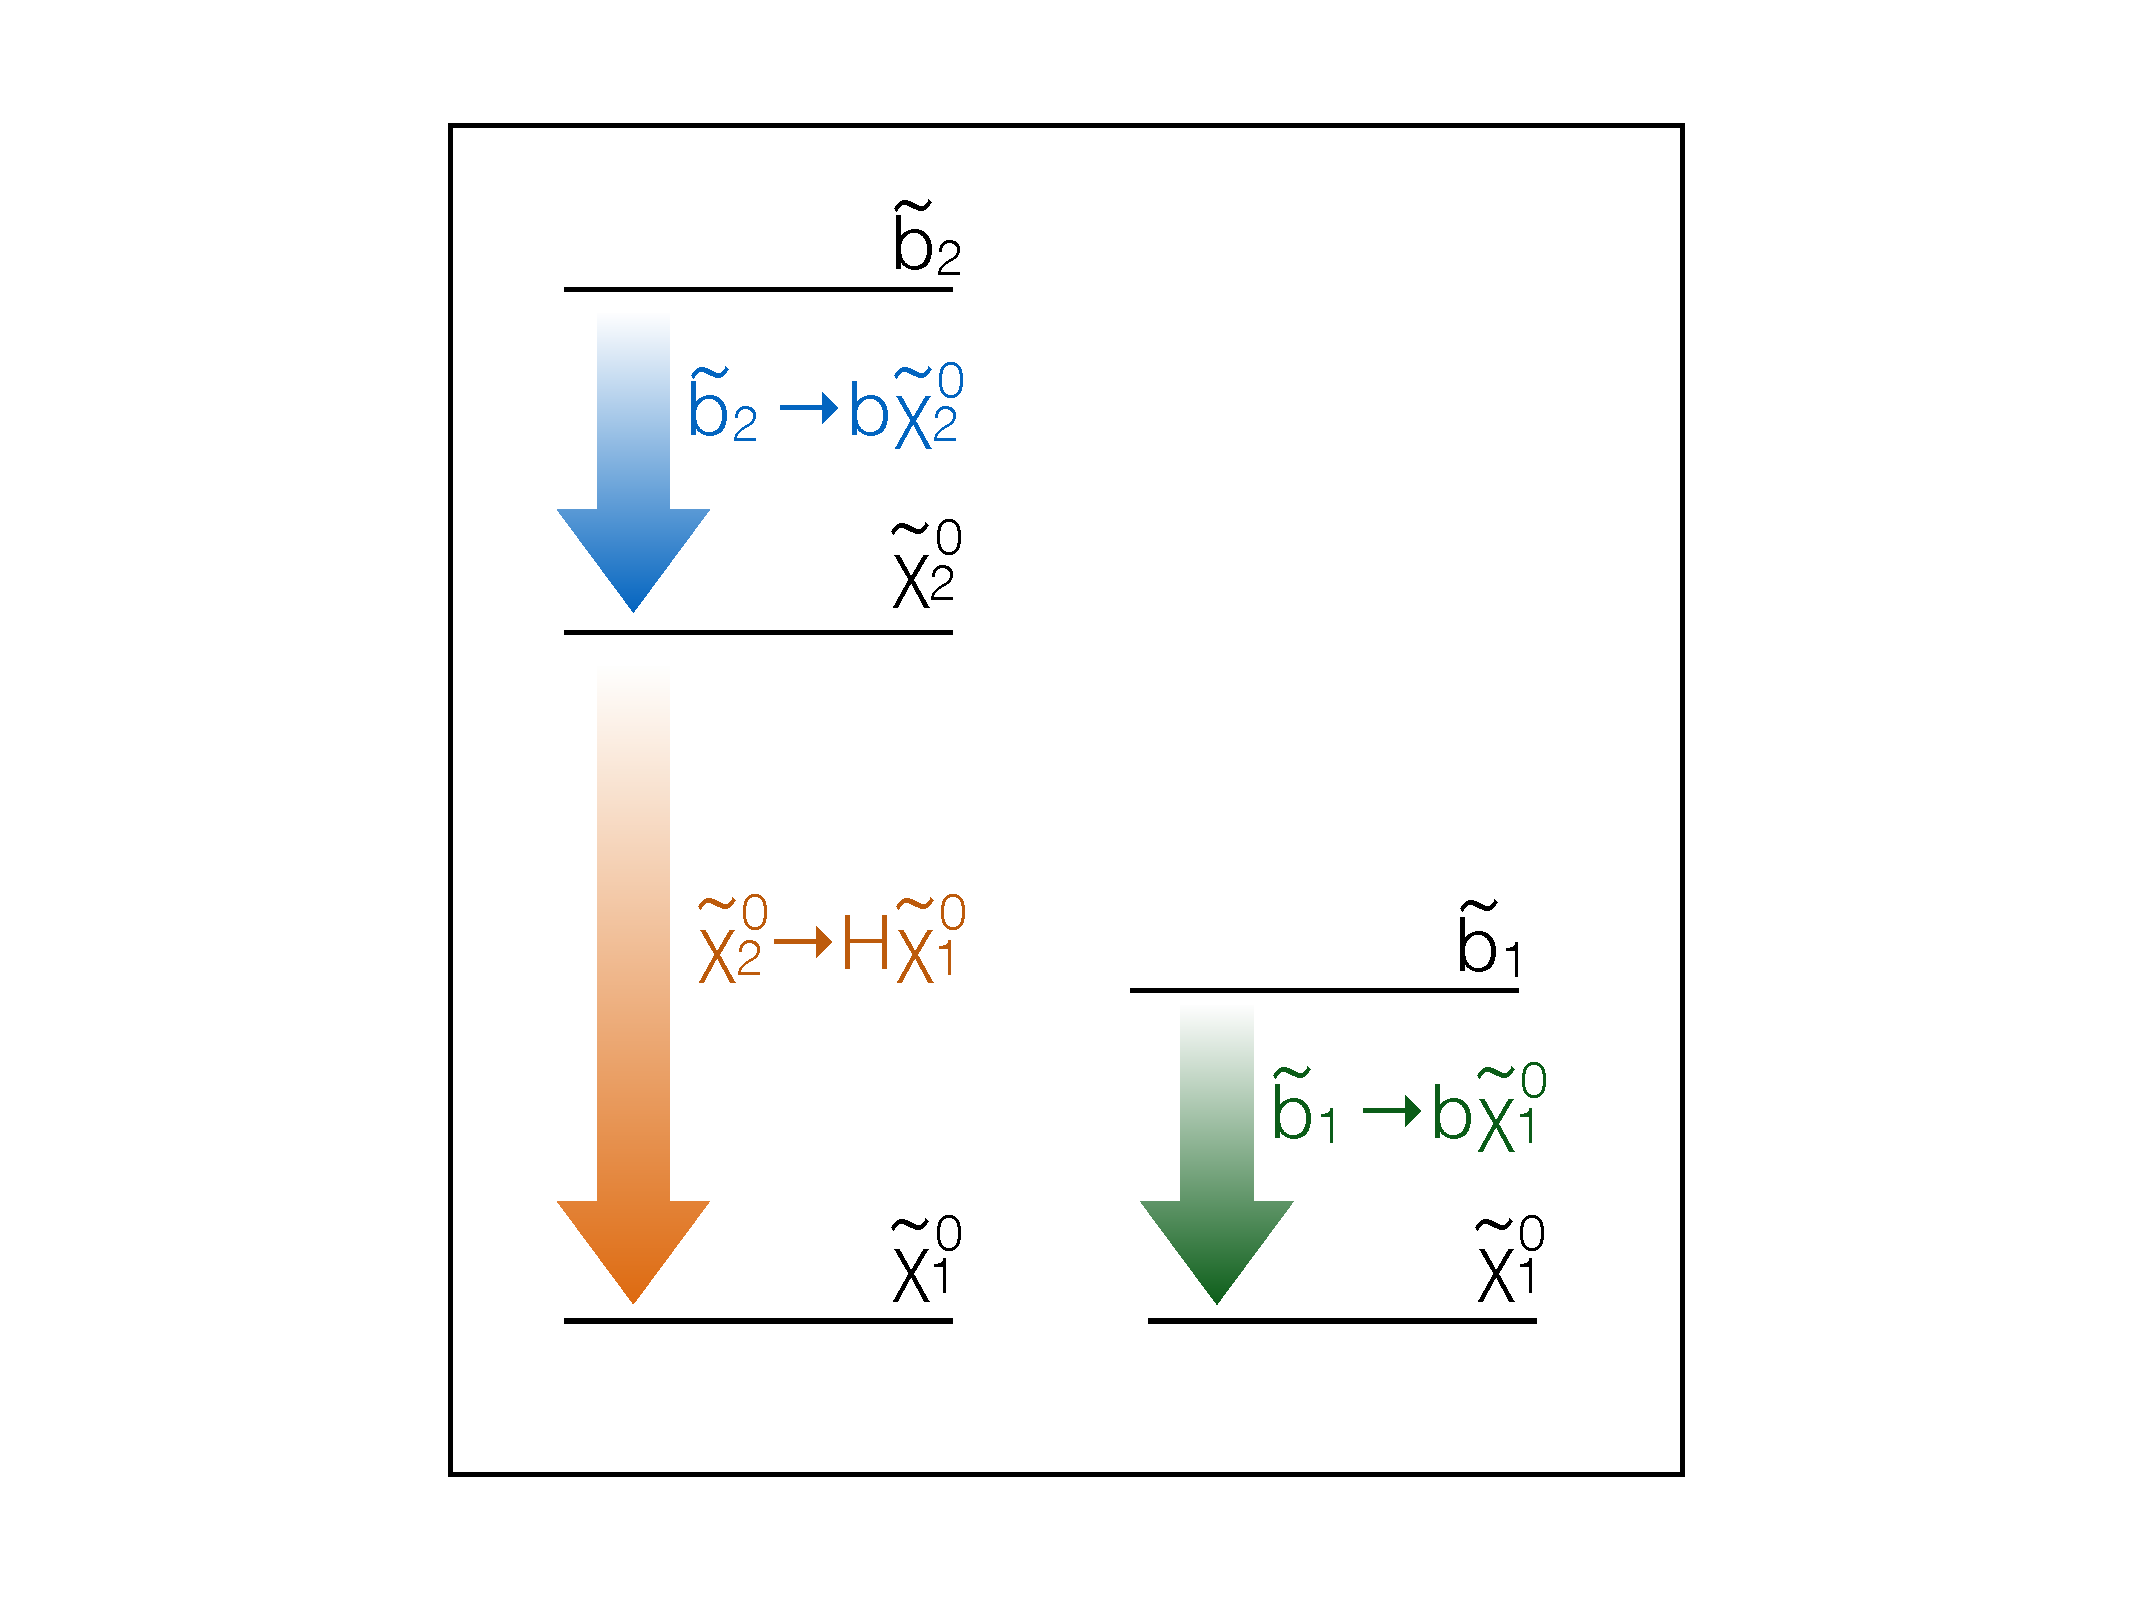
\includegraphics[width=0.23\textwidth,viewport=250 100 800 700,clip=true]{figs/pheno/model1}
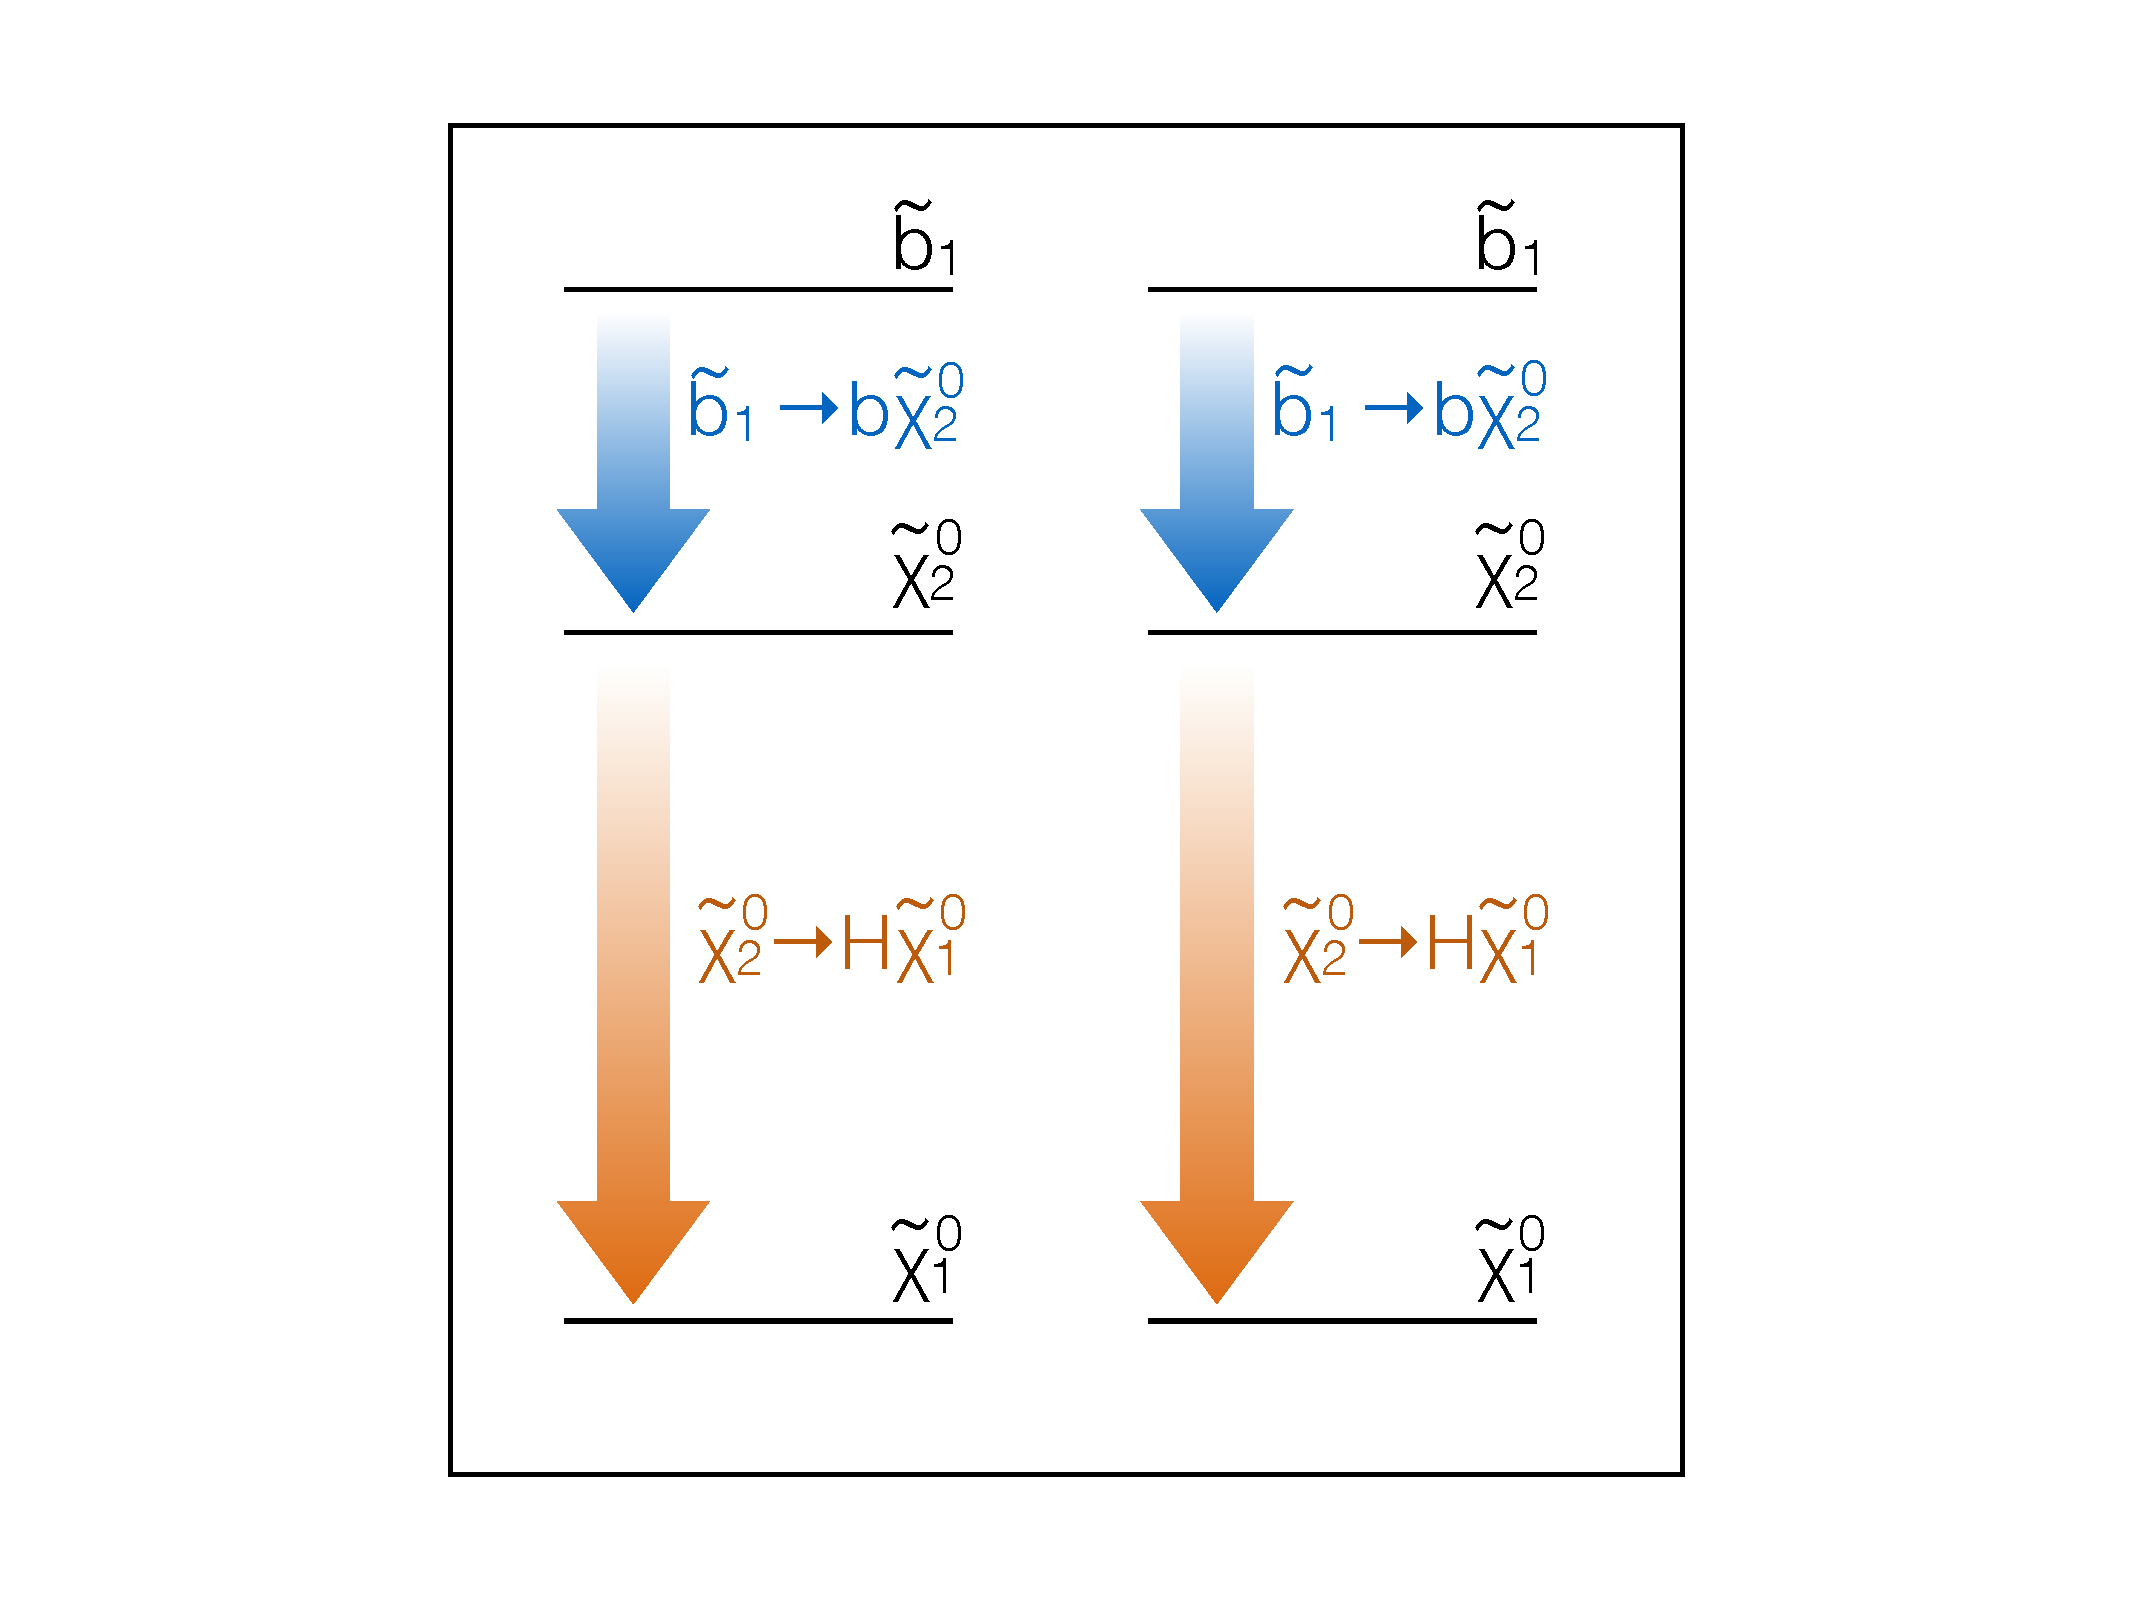
\includegraphics[width=0.23\textwidth,viewport=250 100 800 700,clip=true]{figs/pheno/model2}
\caption{\label{fig:simplifiedModels} Pictorial representation of the
  decay chains associated with model A (left) and model B (right), as described in the text.}
\end{figure}

\section{Event generation and detector simulation}
\label{sec:gensim}
The study is performed using samples of Monte Carlo events. The event generation is performed in \textsc{PYTHIA}~8.210~\cite{Pythia64,Pythia82}.
The default parton density function set is \textsc{NNPDF}~2.3 QCD+QED
LO (with $\alpha_s(M_Z) =
0.130$)~\cite{NNPDF1,NNPDF2,NNPDF3}. Fast simulation of the CMS
detector is performed in \textsc{DELPHES}~3.3.2~\cite{Delphes3}. The
default description of CMS as provided in the release is used, except
for a slight modification to the photon isolation and efficiency,
described in the next section. Jet clustering is performed using
\textsc{FastJet}~3.1.3~\cite{FastJet}. As in CMS, the anti-$k_T$ jet
clustering algorithm is used with jet-size parameter $R=0.5$~\cite{antikt}.

\section{Emulation of the CMS search}
\label{sec:analysis}

The emulated event selection is summarized as follows,
\begin{itemize}
\item Events with two isolated photons with $\pt>25$~GeV and
  $|\eta|<1.44$ are selected. As in Ref.~\cite{CMSPhoton}, the photon
  isolation variables, $I_{\gamma}$, $I_{n}$, and $I_{\pi}$, are
  computed by summing the transverse momenta of photons, neutral
  hadrons, and charged hadrons, respectively, inside an isolation
  cone of radius $\Delta R=0.3$ around the selected photon. The photon
  isolation requirements on these variables
  are shown in Tab~\ref{tab:isolation}. An additional photon selection
  efficiency is applied in \textsc{Delphes} such that isolated photons with $\pt<10$~GeV ($\pt\geq10$~GeV) are
  randomly selected with 94\% (98\%) efficiency.
\begin{table}
\caption{\label{tab:isolation}Photon isolation requirements, as in Ref~\cite{CMSPhoton}.}
%\begin{ruledtabular}
\begin{tabular}{lc|r}
 \multirow{2}{*}{$I_{\gamma}$} & barrel & $1.3~\textrm{GeV} + 0.005\pt^{\gamma}$\\
 & endcap & -- \\\hline
 \multirow{2}{*}{$I_{n}$} & barrel & $3.5~\textrm{GeV} + 0.04\pt^{\gamma}$\\
 & endcap &  $2.9~\textrm{GeV} + 0.04\pt^{\gamma}$ \\\hline
 \multirow{2}{*}{$I_{\pi}$} & barrel & $2.6~\textrm{GeV}$\\
 & endcap &  $2.3~\textrm{GeV}$ \\
\end{tabular}
%\end{ruledtabular}
\end{table}
\item Events with one $\PH$ candidate with $\pt>20$ GeV are selected. A pair of selected
  photons is considered an $\PH$ candidate if at
  least one photon has $\pt>40$~GeV and the diphoton mass
  $m_{\gamma\gamma}>100$~GeV. If the event contains more than one $\PH$ candidate,
  the one with the highest scalar sum $\pt$ of the two photons is selected. 
\item Jets are reconstruted using the \textsc{FastJet}\cite{FastJet} implemtnation
  of the anti-$k_T$\cite{antikt} algorithm with jet radius parameter $R=0.5$.
\item Events with at least one jet with $\pt>30$ GeV and $|\eta|<3.0$
  are selected.
\item An emulation of the medium working point (mistag probability of
  1\% b-tag efficiency of $\sim$ 80\%) of the combined secondary vertex (CSV) b-tagging
  algorithm is used to identify b-jets~\cite{btag8TeV}.
\item A $\bbbar$ candidate pair is identified if both jets satisfy the medium requirement of
  the b-tagging algorithm (note: the CMS analysis requires only one to
  satisfy the medium requirement, while both are required to satisfy
  the loose requirement).
\item The $\bbbar$ candidate pair with the mass closest to 125~GeV or 91.2~GeV is chosen as the $\PH\to
  \bbbar$ or $Z\to \bbbar$ candidate, respectively.
\item The razor variable \MR, calculated from two megajets is required to be greater than
  $150$~GeV. All possible combinations of the reconstructed jets and
the $\PH(\gamma\gamma)$ candidate are clustered to form megajets. The pair of megajets that
minimizes the sum in quadrature of the invariant masses of the two megajets is selected.
\end{itemize}

After this baseline selection, events are categorized according to the
following requirements,
\begin{itemize}
\item \texttt{HighPt}: all events with an $\PH\to\gamma\gamma$ candidate
  with $p_{T}>110$~GeV. 
\item \texttt{Hbb}: remaining events with a $\PH\to b\bar{b}$ candidate
  with mass $110\geq m_{b\bar{b}}\geq 140$~GeV. 
\item \texttt{Zbb}: remaining events with a $Z\to b\bar{b}$ candidate
  with mass $76\geq m_{b\bar{b}}\geq 106$~GeV. 
\item \texttt{HighRes}: 70\% of remaining events (after the \texttt{Zbb} selection). 
\item \texttt{LowRes}: all remaining events. 
\end{itemize}
We assume the breakdown of events between the \texttt{HighRes} box and \texttt{LowRes}
box is 70\%-to-30\% of events after the \texttt{Zbb} selection based on the fact that CMS 
observes a similar breakdown for both SM Higgs background and
electroweak SUSY signal processes in Monte Carlo simulation~\cite{RazorHgaga}.

%Given the difficulty of emulating the high-resolution requirement
%(both photons must satisfy $\sigma_E/E<0.015$, where $\sigma_E/E$ is the relative
%energy resolution for the identified photons) for the \texttt{HighRes}
%box, and the high efficiency of this requirement for \emph{real}
%photons, we make the assumption that all of our benchmark signal events (which contain
%a real $\PH\to\gamma\gamma$) pass this requirement and thus no signal events
%fall into the \texttt{LowRes} box.

Finally, the search region selection is as follows,
\begin{itemize}
\item The search region in the $m_{\gamma\gamma}$ distribution is
    defined by $(125 - 2\sigma_{\mathrm{eff}},
    126+2\sigma_{\mathrm{eff}})$ in each event category, where
    $\sigma_{\mathrm{eff}}$ is defined such that $\sim68\%$ of Higgs
    boson events fall in an interval of $\pm\sigma_{\mathrm{eff}}$
    around the nominal $m_H$ value. Using this procedure, we derive
    $\sigma_{\mathrm{eff}}$ to be 3.8~GeV in the \texttt{HighRes} box
    and 2.2~GeV in the  \texttt{HighRes} and \texttt{LowRes}
    boxes. For the \texttt{Hbb} and \texttt{Zbb} boxes, we use the overall average value
    of 2.8~GeV as in Ref.~\cite{RazorHgaga}.
    %$\sigma_{\mathrm{eff}}=1.46$~GeV in the \texttt{HighRes} box, 
   %$\sigma_{\mathrm{eff}}=1.56$~GeV in the \texttt{HighPt} box, and $\sigma_{\mathrm{eff}}=2$~GeV in the
%\texttt{Hbb} and \texttt{Zbb} boxes.
\end{itemize}

\subsection{Bayesian Statistical Interpretation}
We model the likelihood according to a Poisson density,
considering the expected background yield (with associated
uncertainty), the expected signal yield (for a given signal cross
section), and the observed yield. The background uncertainty is modeled with a gamma density. The
background yields and the corresponding uncertainties are taken from the tables provided
in Ref.~\cite{RazorHgaga}. To take into account systematic
uncertainties on the signal, we assign a 30\% uncertainty (assuming a
log-normal density) on the signal strength, a multiplicative
factor modifying the signal cross section. We then derive the
posterior density for the signal cross section $\sigma$ as:
\begin{eqnarray}
p(\sigma|\mathrm{data}) &\propto& \mathcal L(\mathrm{data} |\sigma)
                                  p_0(\sigma)
\label{eqn:posterior}
\end{eqnarray}
where $\mathcal L(\mathrm{data} |\sigma)$ is the likelihood and $p_0(\sigma)$ is the prior density taken to be
flat. The likelihood is then
\begin{eqnarray}
\mathcal L(\mathrm{data} |\sigma) &=&\int_{0}^{\infty}d\mu~\mathrm{Ln}(\mu|\bar\mu,\delta\mu)\nonumber\\
&&\times\prod_{i=0}^{n_{\mathrm{bins}}}\int_0^{\infty} db_i~
   \mathrm{Poisson}(n_i|L\mu\sigma\epsilon_i+ b_i)\nonumber\\
&&\times~\mathrm{Gamma}(b|\bar{b}_i,\delta b_i)
\label{eqn:likelihood}
\end{eqnarray}
where the product runs over the number of bins $n_{\mathrm{bins}}$; $n_i$ is the
observed yield in the $i^{\mathrm{th}}$ bin, $L$ is the integrated
luminosity, $b_i$ is the actual value of the background yield in the
$i^{\mathrm{th}}$ bin and $\bar{b}_i\pm \delta b_i$ is its expected value
and the associated uncertainty; $\epsilon_i$ is the nominal value
of the signal efficiency in the $i^{\mathrm{th}}$ bin; $\mu$ is the
signal strength, a nuisance parameter modifying the signal cross section
(nominally equal to $\bar\mu=1$ with a $\delta\mu=30\%$ uncertainty);
$\mathrm{Ln}(x|m,\delta)$ is the log-normal
distribution for $x$, parameterized such that $\mathrm{log}(m)$ is the
mean and $\mathrm{log}(1+m\delta)$ is the standard deviation of the
log of the distribution; $\mathrm{Gamma}(x|m,\delta)$ is the gamma
distribution for $x$, parameterized such that $m$ is the
mode and $\delta^2$ is the variance of the distribution. The 95\%
credibility level (CL) upper limit on the
signal cross section $\sigma_{\mathrm{up}}$ is obtained from the
posterior, such that 
\begin{equation}
\frac{\int_0^{\sigma_{\mathrm{up}}}d\sigma~ p(\sigma|\mathrm{data})}{\int_0^{\infty}d\sigma~ p(\sigma|\mathrm{data})} = 0.95~.
\end{equation}

We also utilize a signal significance measure defined by
\begin{eqnarray}
Z(\sigma) &=& \mathrm{sign}[\log B_{10}(\mathrm{data},\sigma)]\sqrt{2|\log B_{10}(\mathrm{data},\sigma)|}
\label{eqn:zSig}
\end{eqnarray}
where 
\begin{eqnarray}
B_{10}(\mathrm{data},\sigma) &=& \frac{\mathcal L(\mathrm{data}
  |\sigma,H_1)}{\mathcal L(\mathrm{data}
  |H_0)}
\label{eqn:localBayes}
\end{eqnarray}
is the \emph{local} Bayes factor for the data for a given signal cross
section $\sigma$, and $\mathcal L(\mathrm{data}
  |\sigma,H_1)$ and $\mathcal L(\mathrm{data}
  |H_0)$ are the likelihoods for the signal-plus-background ($H_1$) and
  background-only ($H_0$) hypotheses, respectively. As described in
  Ref.~\cite{CMS-PAS-SUS-15-010}, this
  measured is a signed Bayesian analog of the frequentist ``n-sigma.''
  For each signal model with specified masses, we scan the siganl
  cross section $\sigma$ to find the maximum significance,
  which occurs at the mode of the posterior.
\subsection{Cross-validation and Correction}
To cross-validate our emulation result, we produced 95\% CL
limits on the production cross section of an electroweak simplified
model of $\tilde{\chi}_1^{\pm}\tilde{\chi}_2^0$ production, followed by
the decays $\tilde{\chi}_1^{\pm}\to W^{\pm}\tilde\chi_1^0$,
$\tilde{\chi}_2^0\to H\chi_1^0$. For this model, CMS provided the 95\%
confidence level upper limits on the cross section assuming an LSP mass of
$m_{\tilde\chi_1^0}=1$~GeV and equal chargino and second neutralino
masses, $m_{\tilde{\chi}_1^{\pm}}=m_{\tilde{\chi}_2^0}$. 
%The posterior density
%for the production cross sections (assuming
%$m_{\tilde{\chi}_1^{\pm}}=200$~GeV) derived from our emulation of the CMS search are shown in
%figure~\ref{fig:TChiwhPosterior200}. 
The comparison between our result and the CMS result for this model is shown in
figure~\ref{fig:TChiwh1dLimit} as a function of $m_{\tilde{\chi}_1^{\pm}}$.

%The expected upper limit from the emulation is consistently larger
%than the expected upper limit from the CMS result by a
%factor of $1.2$, $1.3$, and $1.5$ for $m_{\tilde{\chi}_1^{\pm}}
%=130$~GeV, $160$~GeV, and $200$~GeV, respectively. Similarly, the
%corresponding ratio of the observed upper limits are $1.4$, $1.7$, and
%$2.3$ for $m_{\tilde{\chi}_1^{\pm}}=130$~GeV, $160$~GeV, and $200$~GeV, respectively.

%\begin{figure}[htb]
%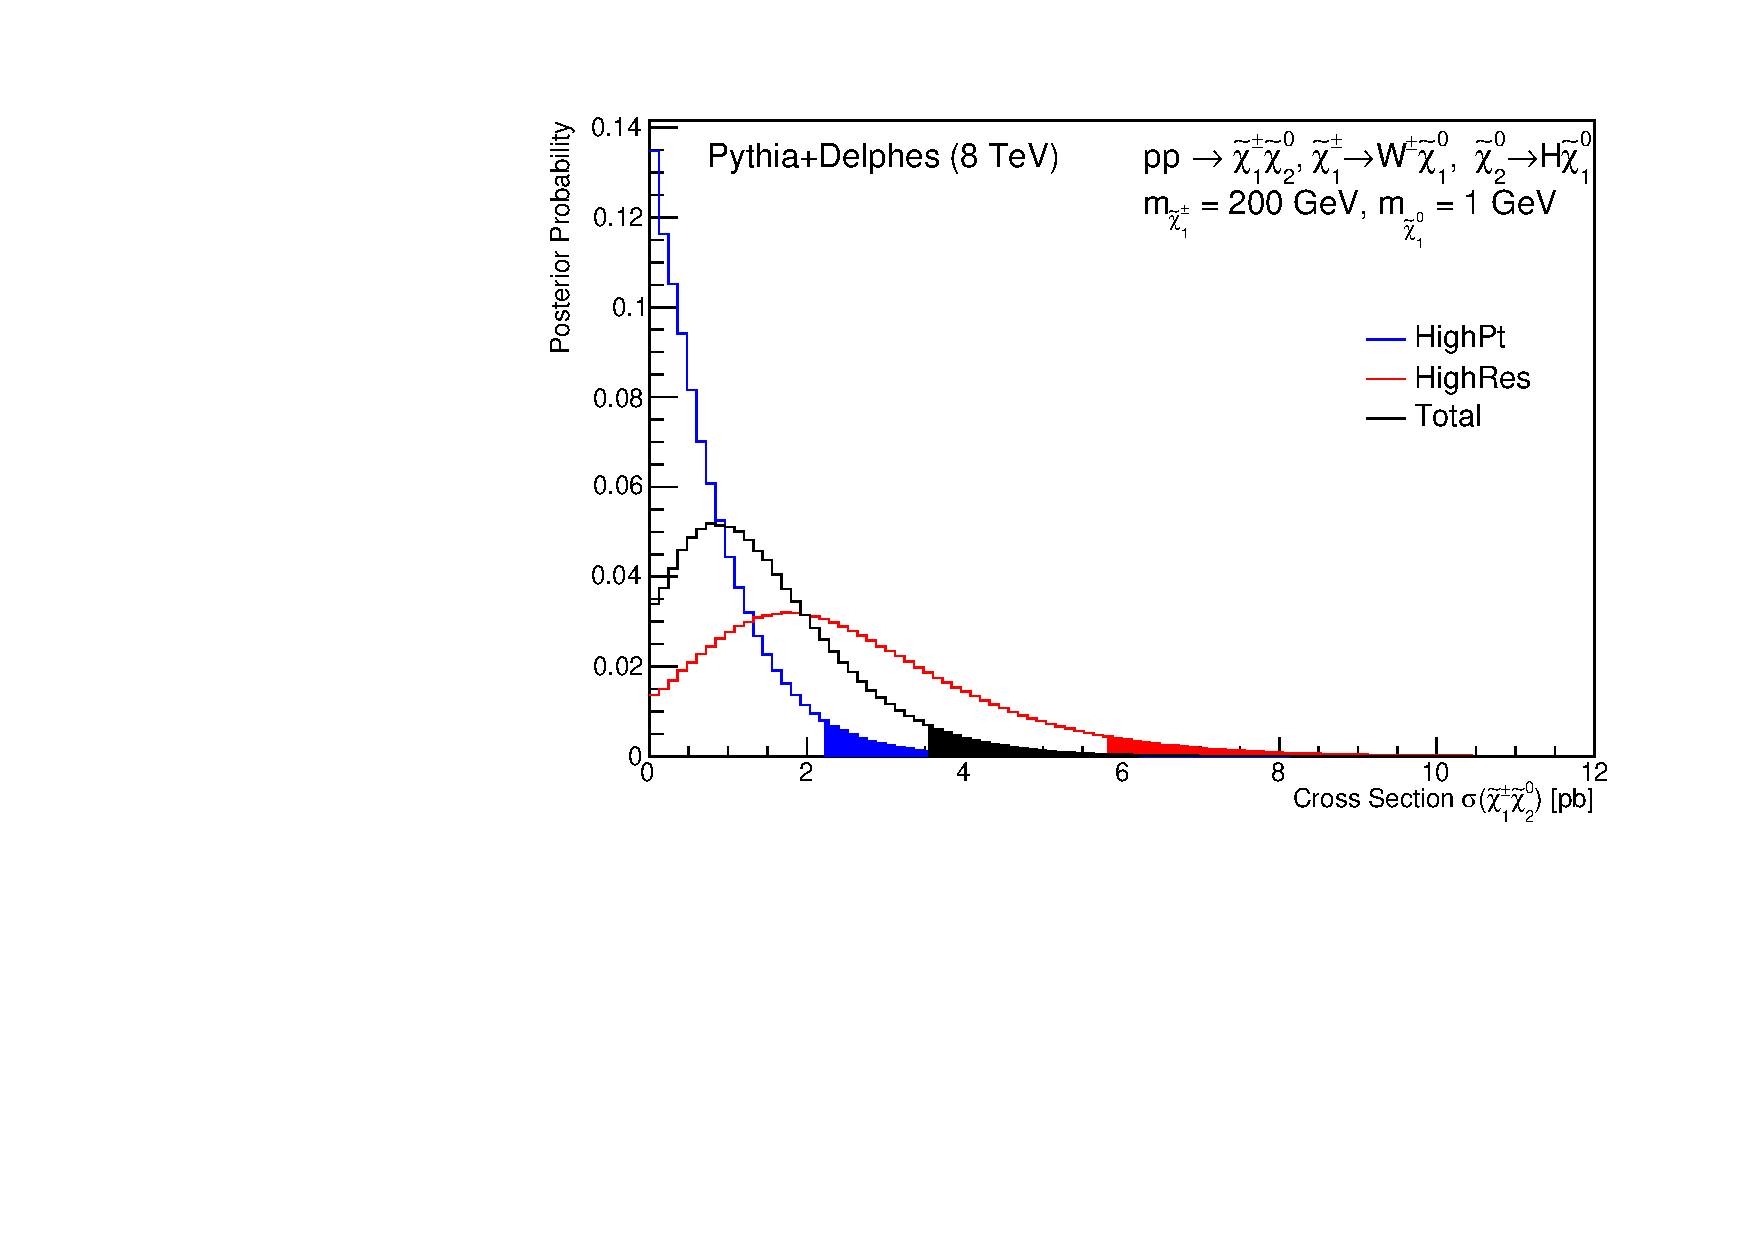
\includegraphics[width=0.45\textwidth]{figs/pheno/posterior_TChiwh_200_1.pdf}
%\caption{\label{fig:TChiwhPosterior200} Posterior probability
 % density functions for the production cross section for the \texttt{HighPt}
 % box (blue), \texttt{HighRes} box (red), and the combination (black). The solid colored region
 % under each curve illustrates the 5\% tail probability. Note, the chosen masses are $m_{\tilde\chi_1^0}=1$~GeV and
 % $m_{\tilde{\chi}_1^{\pm}}=m_{\tilde{\chi}_2^0}=200$~GeV.}
%\end{figure}

\begin{figure}[htb]
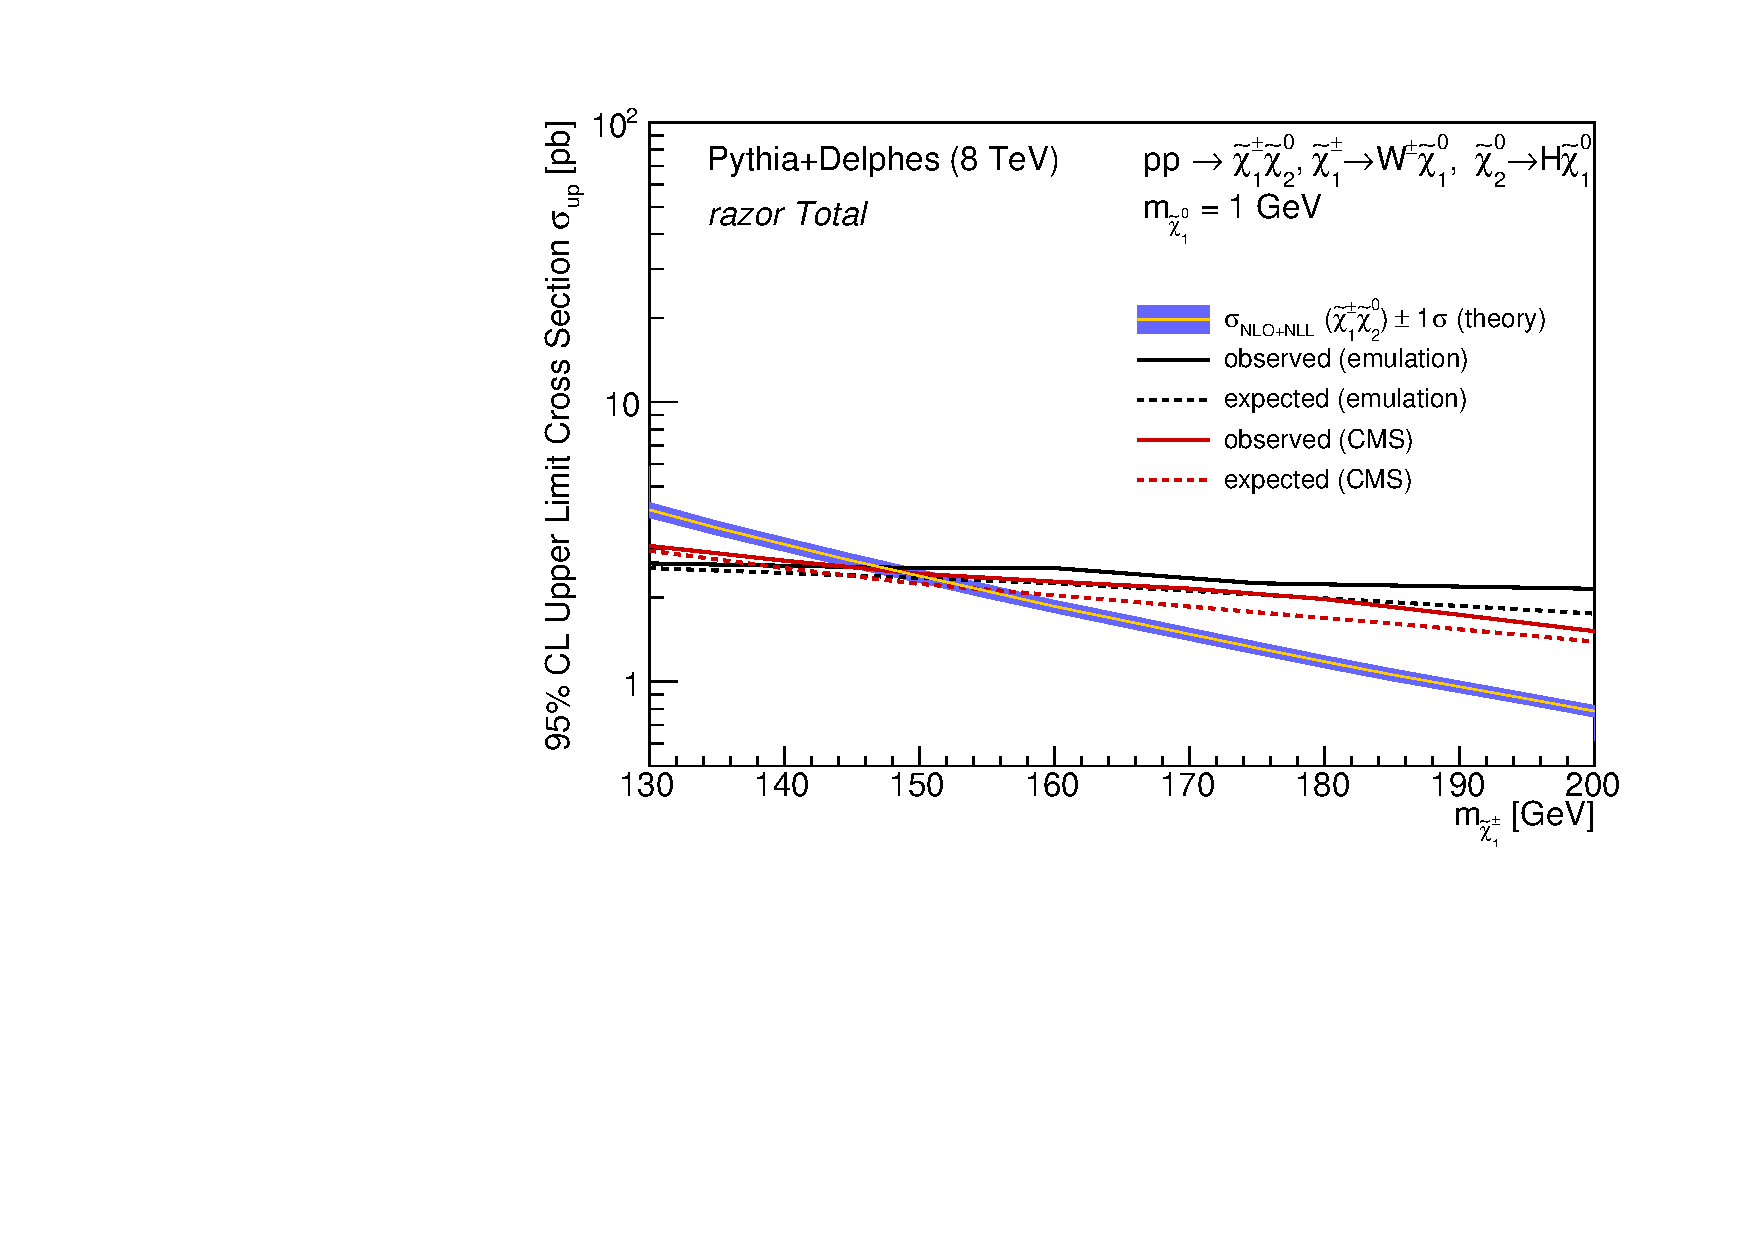
\includegraphics[width=0.45\textwidth]{figs/pheno/xsecUL_TChiwh_1_Total.pdf}
\caption{\label{fig:TChiwh1dLimit} Comparison between the CMS
 result (red) and our emulation (black). Note, this scan assumes
 $m_{\tilde\chi_1^0}=1$~GeV and $m_{\tilde{\chi}_1^{\pm}}=m_{\tilde{\chi}_2^0}$.}
\end{figure}


\section{Results}
\label{sec:results}

%Fig.~\ref{fig:T21bHPosterior500}  shows the posteriors for different
%boxes and the combination for a particular mass point in model
%A ($m_{\sbottom_2}=500$~GeV, $m_{\sbottom_2}=130$~GeV,
%$m_{\chiztwo}=230$~GeV, and $m_{\chizone}=130$~GeV). 
To show how well signal model A agrees with the excess,
Fig.~\ref{fig:T21bHExpObs500800} displays the expected SM background
distribution and uncertainty compared to the distribution of the
signal events for $m_{\sbottom_2}=500$~GeV and
$m_{\sbottom_2}=800$~GeV, with other mass paramters set as
$m_{\sbottom_2}=130$~GeV, $m_{\chiztwo}=230$~GeV, and
$m_{\chizone}=130$~GeV. The bin numbers correspond to the order given
in the yield tables in Ref.~\cite{RazorHgaga}. %to Tab.~\ref{tab:bins}.
%\begin{table}[htb] \centering
%\caption{\label{tab:bins}\texttt{HighRes} bin numbering scheme.}
%\begin{tabular}{|c|cc|}
%\hline
%Bin &\MR~range & \Rsq~range \\
%\hline
% 0 &  150 -    250 & 0.00 - 0.05\\
% 1 & 150 -    250 & 0.05 - 0.10\\
% 2 & 150 -    250 & 0.10 - 0.15\\
% 3 &  150 -    250 & 0.15 - 1.00\\
% 4 &  250 -    400 & 0.00 - 0.05\\
% 5 &  250 -    400 & 0.05 - 0.10\\
% 6 &  250 -    400 & 0.10 - 1.00\\
% 7 & 400 -   1400 & 0.00 - 0.05\\
% 8 &  400 -   1400 & 0.05 - 1.00\\
% 9 & 1400 -   3000 & 0.00 - 1.00\\
%\hline
%\end{tabular}
%\end{table}
The normalization for the signal is
taken from the mode (i.e. ``best-fit'') signal cross section of the posterior density in the
\texttt{HighRes} box. Fainlly, Fig.~\ref{fig:T21bH1dLimit}, shows the
95\% CL combined limit as a function of the $\sbottom_2$ mass.


%Fig.~\ref{fig:T2bHPosterior450},~\ref{fig:T2bHExpObs450800},~and~\ref{fig:T2bH1dLimit}
%are
Fig.~\ref{fig:T2bHExpObs500800},~and~\ref{fig:T2bH1dLimit} are
the analagous results for model B. The chosen model B mass points in Fig.~\ref{fig:T2bHExpObs500800} are
$m_{\sbottom_1}=500$~GeV or $m_{\sbottom_1}=800$~GeV , $m_{\chiztwo}=230$~GeV, and
$m_{\chizone}=130$~GeV and the limit scan in Fig.~\ref{fig:T2bH1dLimit} is as a function of the $\sbottom_1$ mass.

%\begin{figure}[htb]
%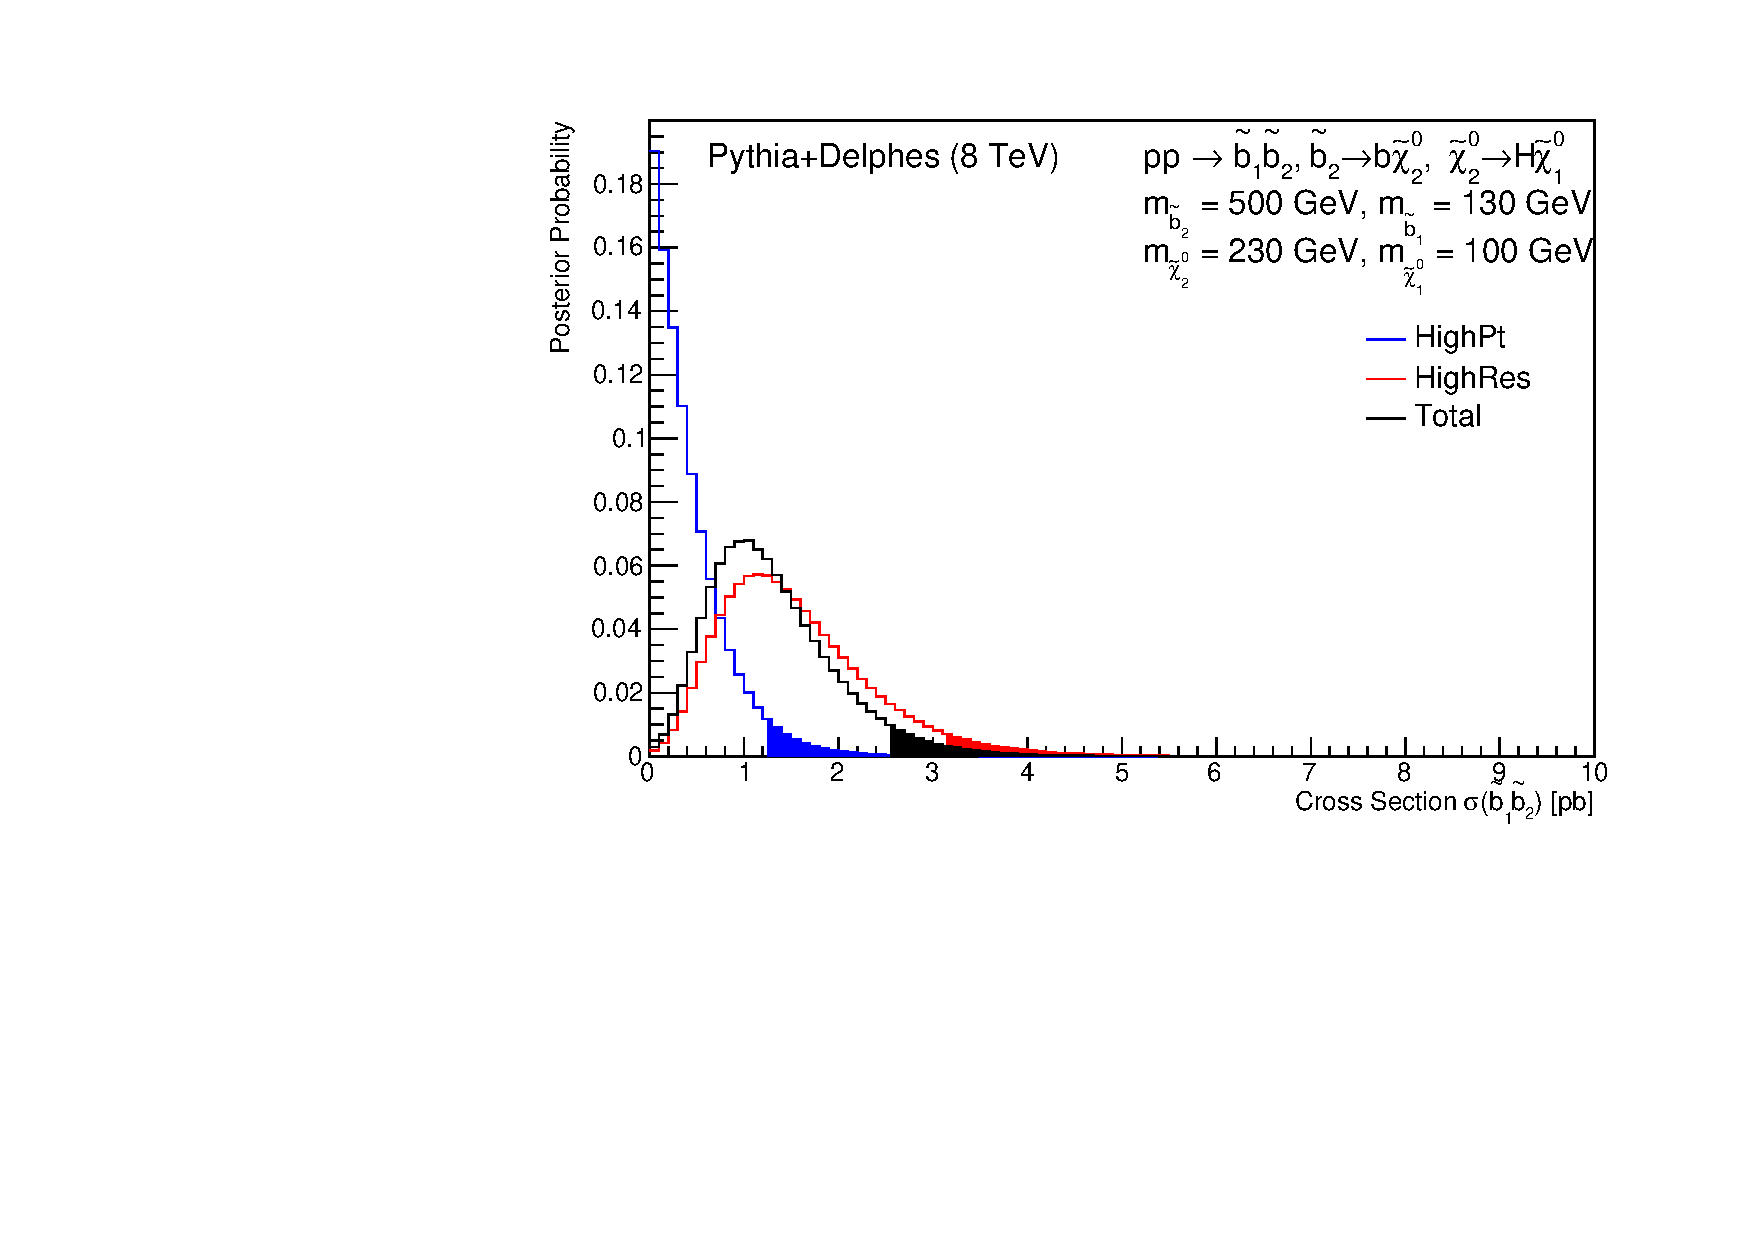
\includegraphics[width=0.45\textwidth]{figs/pheno/posterior_T21bH_500_130_100.pdf}
%\caption{\label{fig:T21bHPosterior500} Posterior probability
 % density functions for the $\sbottom_1\sbottom_1$ production cross
 % section in model A for the \texttt{HighPt} box (blue), \texttt{HighRes} box (red), and the combination (black). The solid colored region
 % under each curve illustrates the 5\% tail probability. Note, the chosen masses are $m_{\tilde\chi_1^0}=100$~GeV and
 % $m_{\tilde{\chi}_2^0}=230$~GeV.}
%\end{figure}

\begin{figure}[htb]
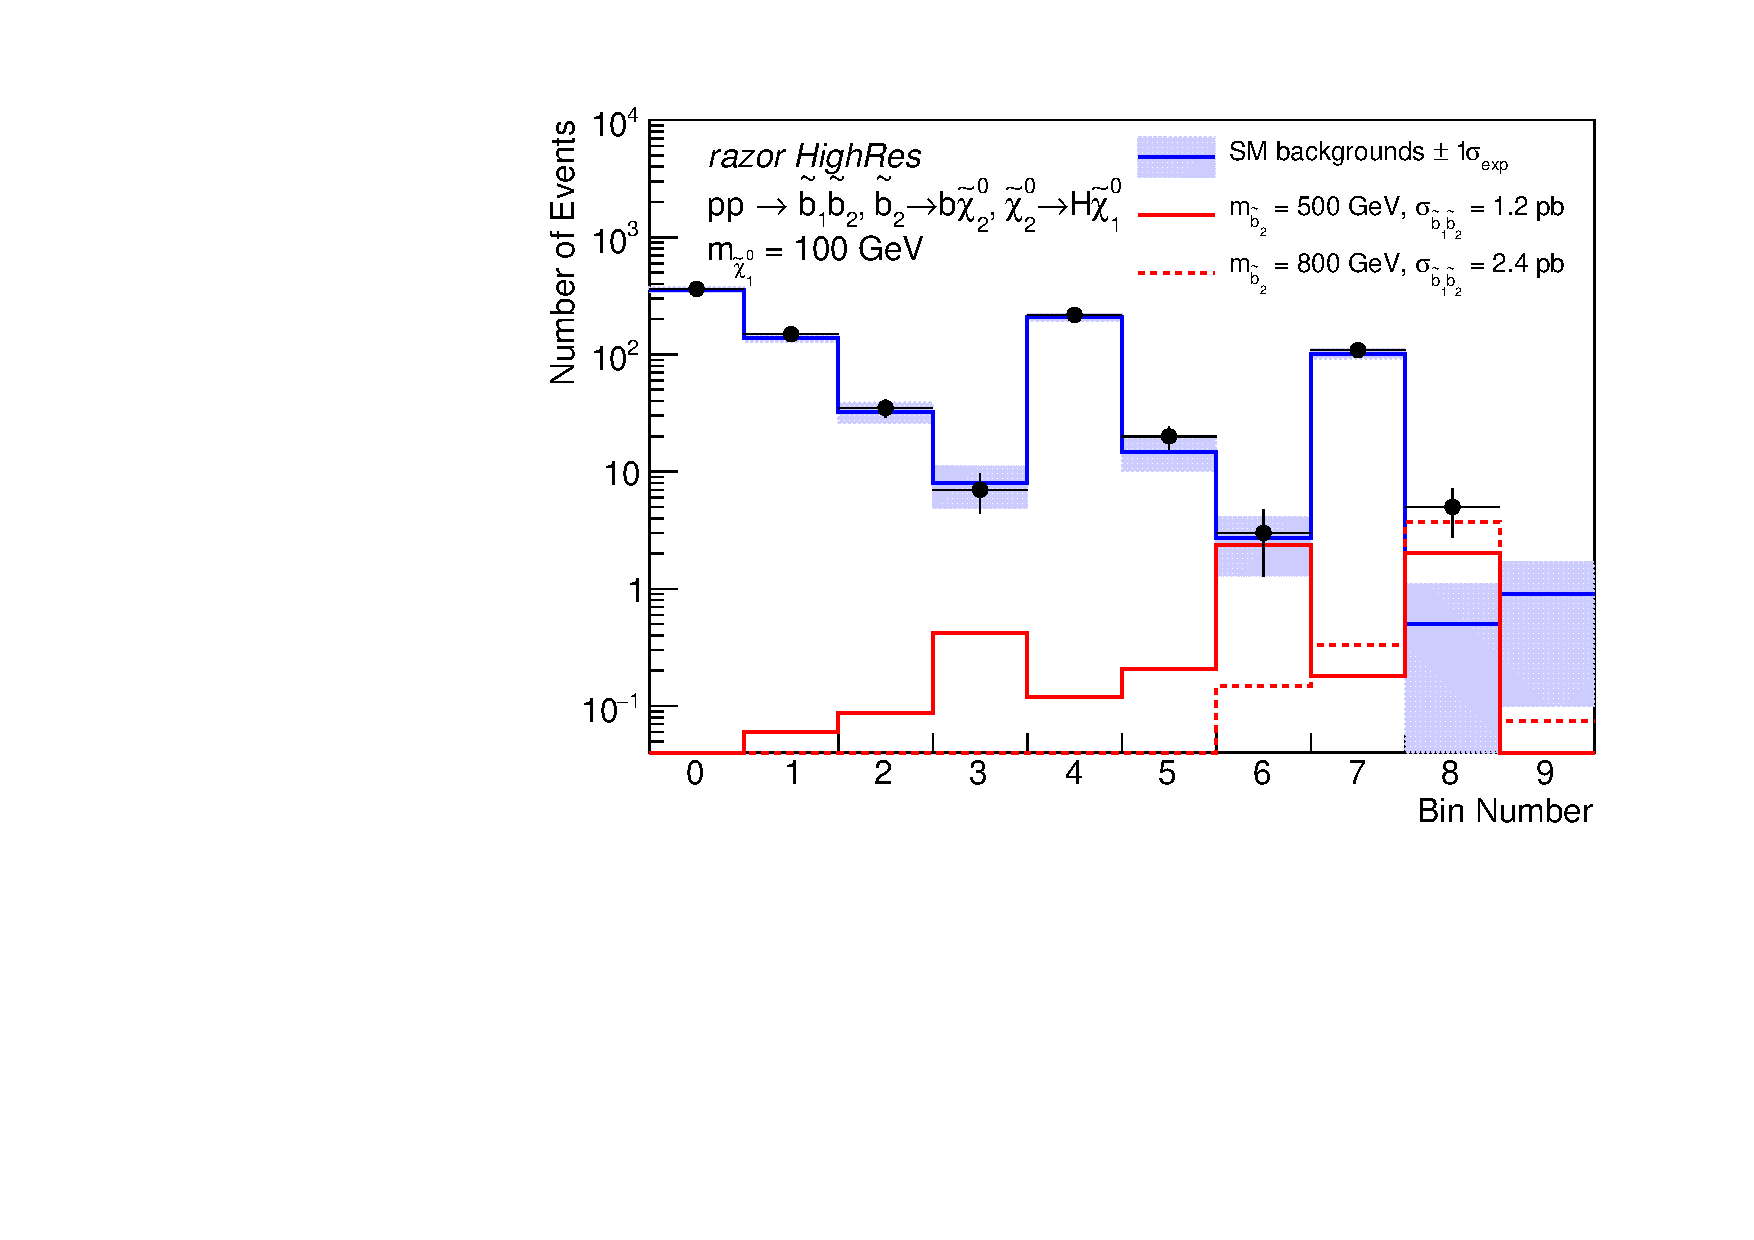
\includegraphics[width=0.45\textwidth]{figs/pheno/obsexp_T21bH_HighRes.pdf}
\caption{\label{fig:T21bHExpObs500800} The expected background and
  uncertainty compared to the ``best-fit'' signal distribution in the \texttt{HighRes} box for two particular
  mass points, $m_{\sbottom_2}=500$~GeV and $m_{\sbottom_2}=800$~GeV, in model A.}
\end{figure}

\begin{figure}[htb]
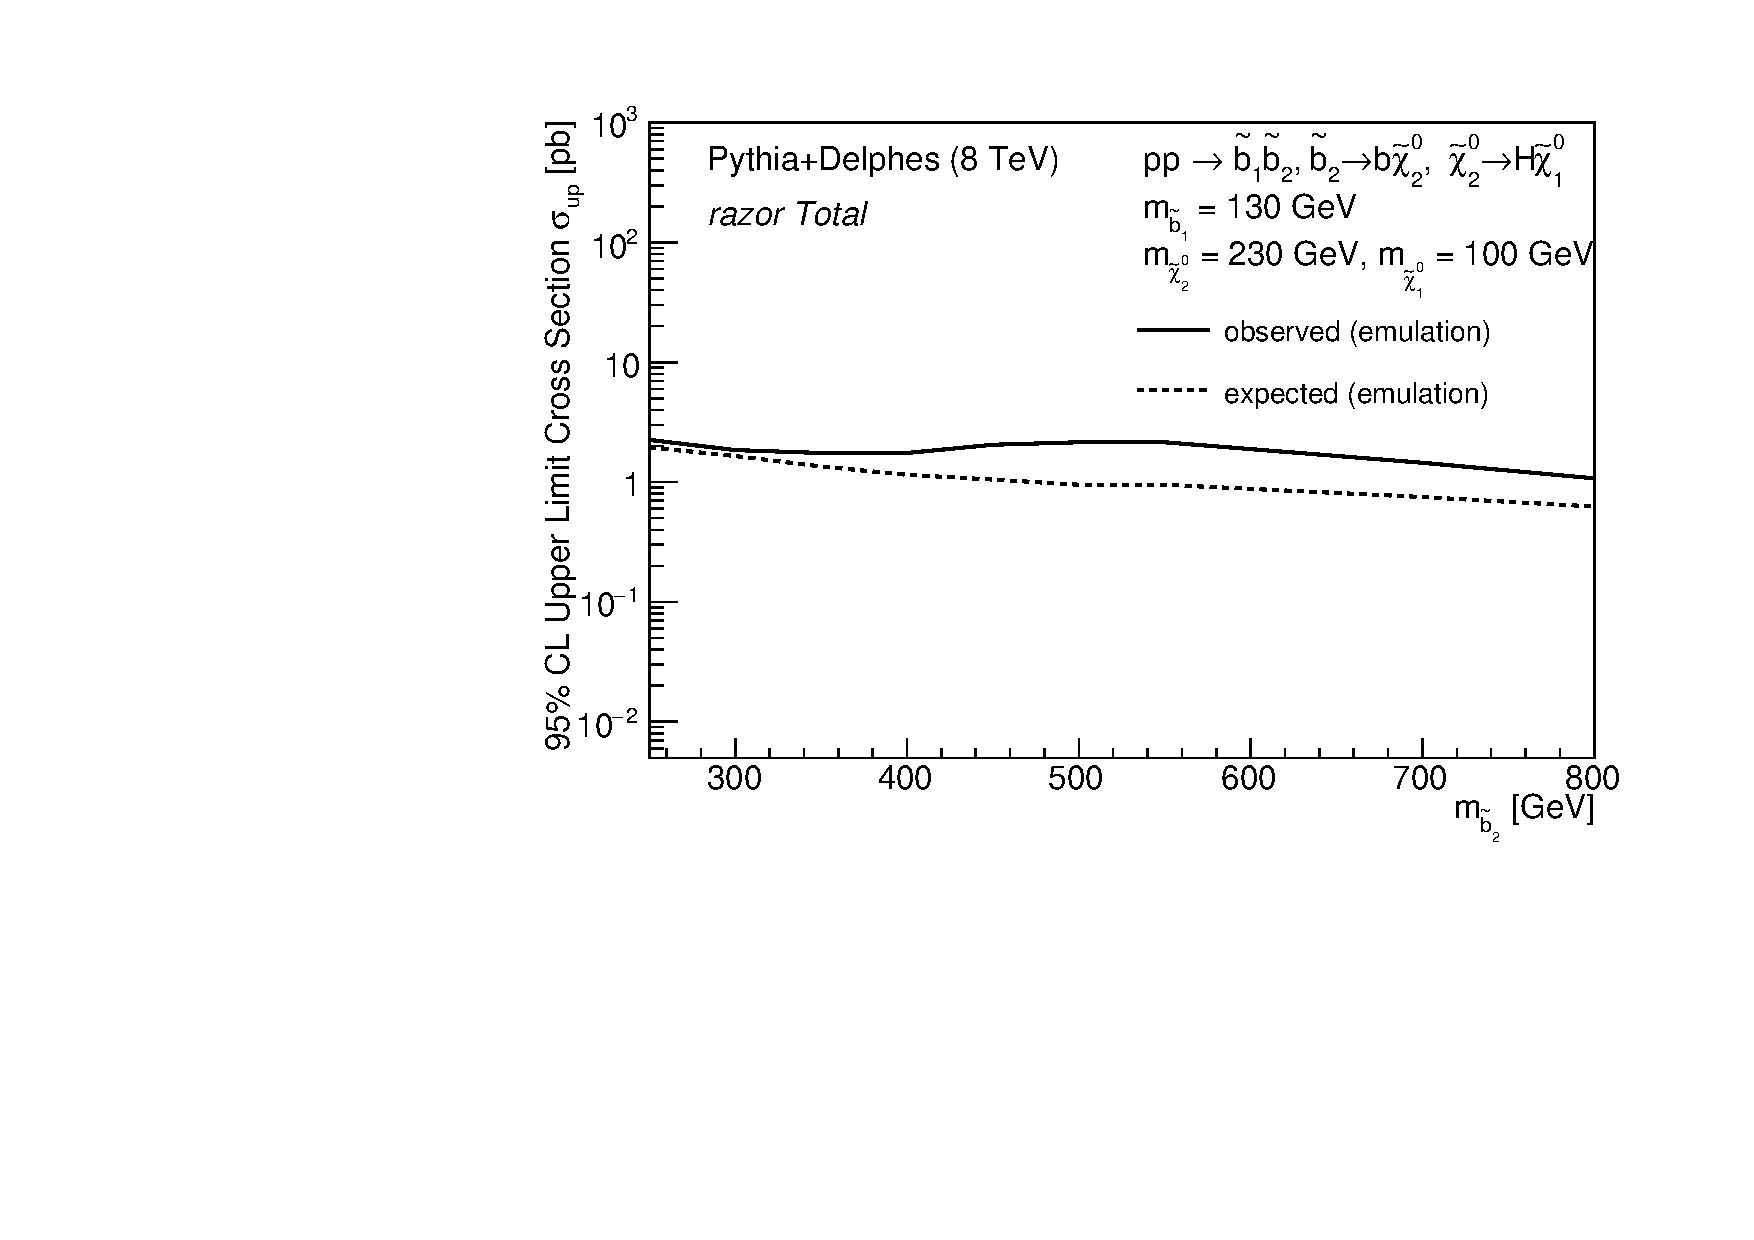
\includegraphics[width=0.45\textwidth]{figs/pheno/xsecUL_T21bH_130_100_Total.pdf}
\caption{\label{fig:T21bH1dLimit} The 95\% CL upper limit on the
  cross section on $\sbottom_1\sbottom_2$ production in model A as a function of $m_{\sbottom_2}$ (black) compared
  to the LO predicted cross section (yellow). Note, this scan assumes
  $m_{\tilde\chi_1^0}=100$~GeV, $m_{\tilde{\chi}_2^0}=230$~GeV, and  $m_{\sbottom_1}=130$~GeV.}
\end{figure}

\begin{figure}[htb]
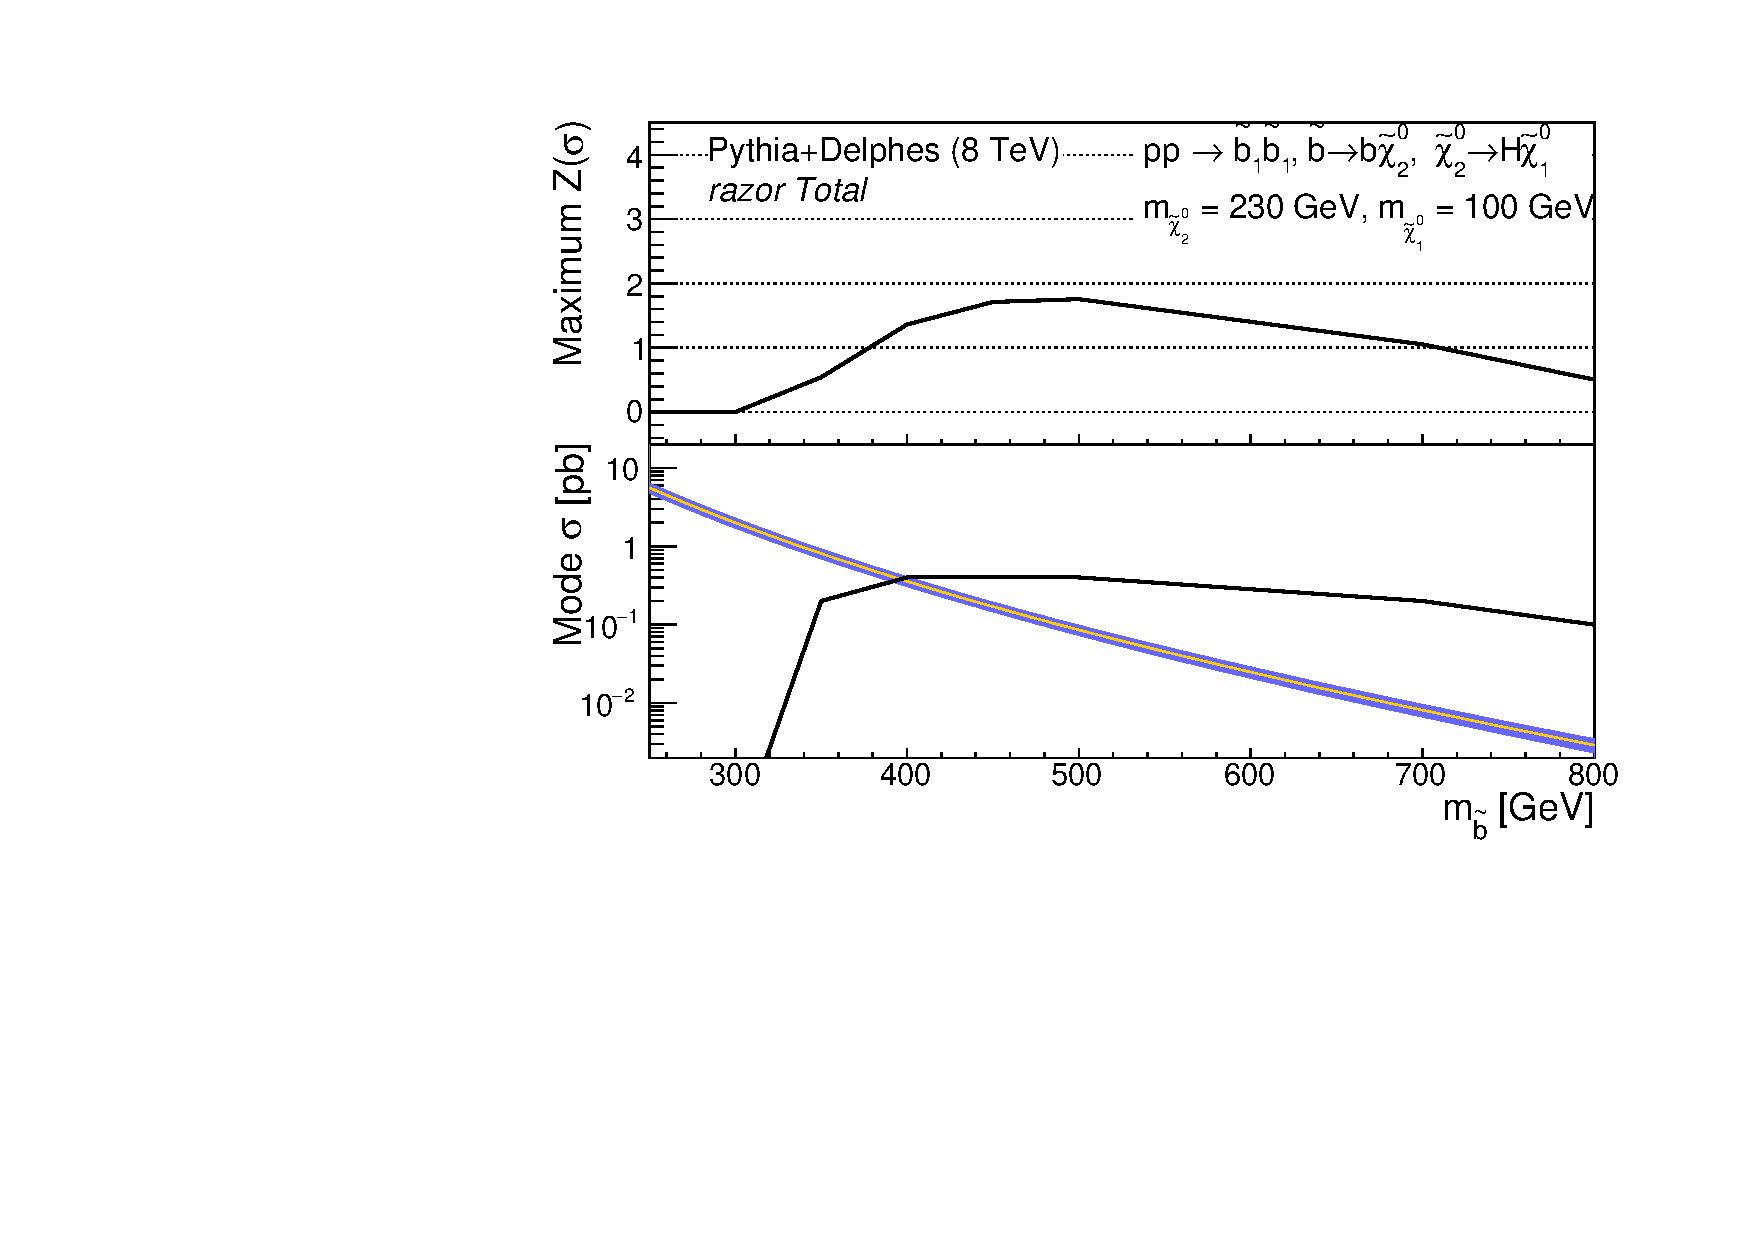
\includegraphics[width=0.45\textwidth]{figs/pheno/signif_T2bH_100_Total.pdf}
\caption{\label{fig:T21bH1dSignif} The maximum significance $Z$ for a
  given $m_{\sbottom_2}$ (top) and the ``best fit'' signal cross
  section (bottom). Note, this scan assumes
  $m_{\tilde\chi_1^0}=100$~GeV, $m_{\sbottom_1}=130$~GeV  and $m_{\tilde{\chi}_2^0}=230$~GeV.}
\end{figure}

%\begin{figure}[htb]
%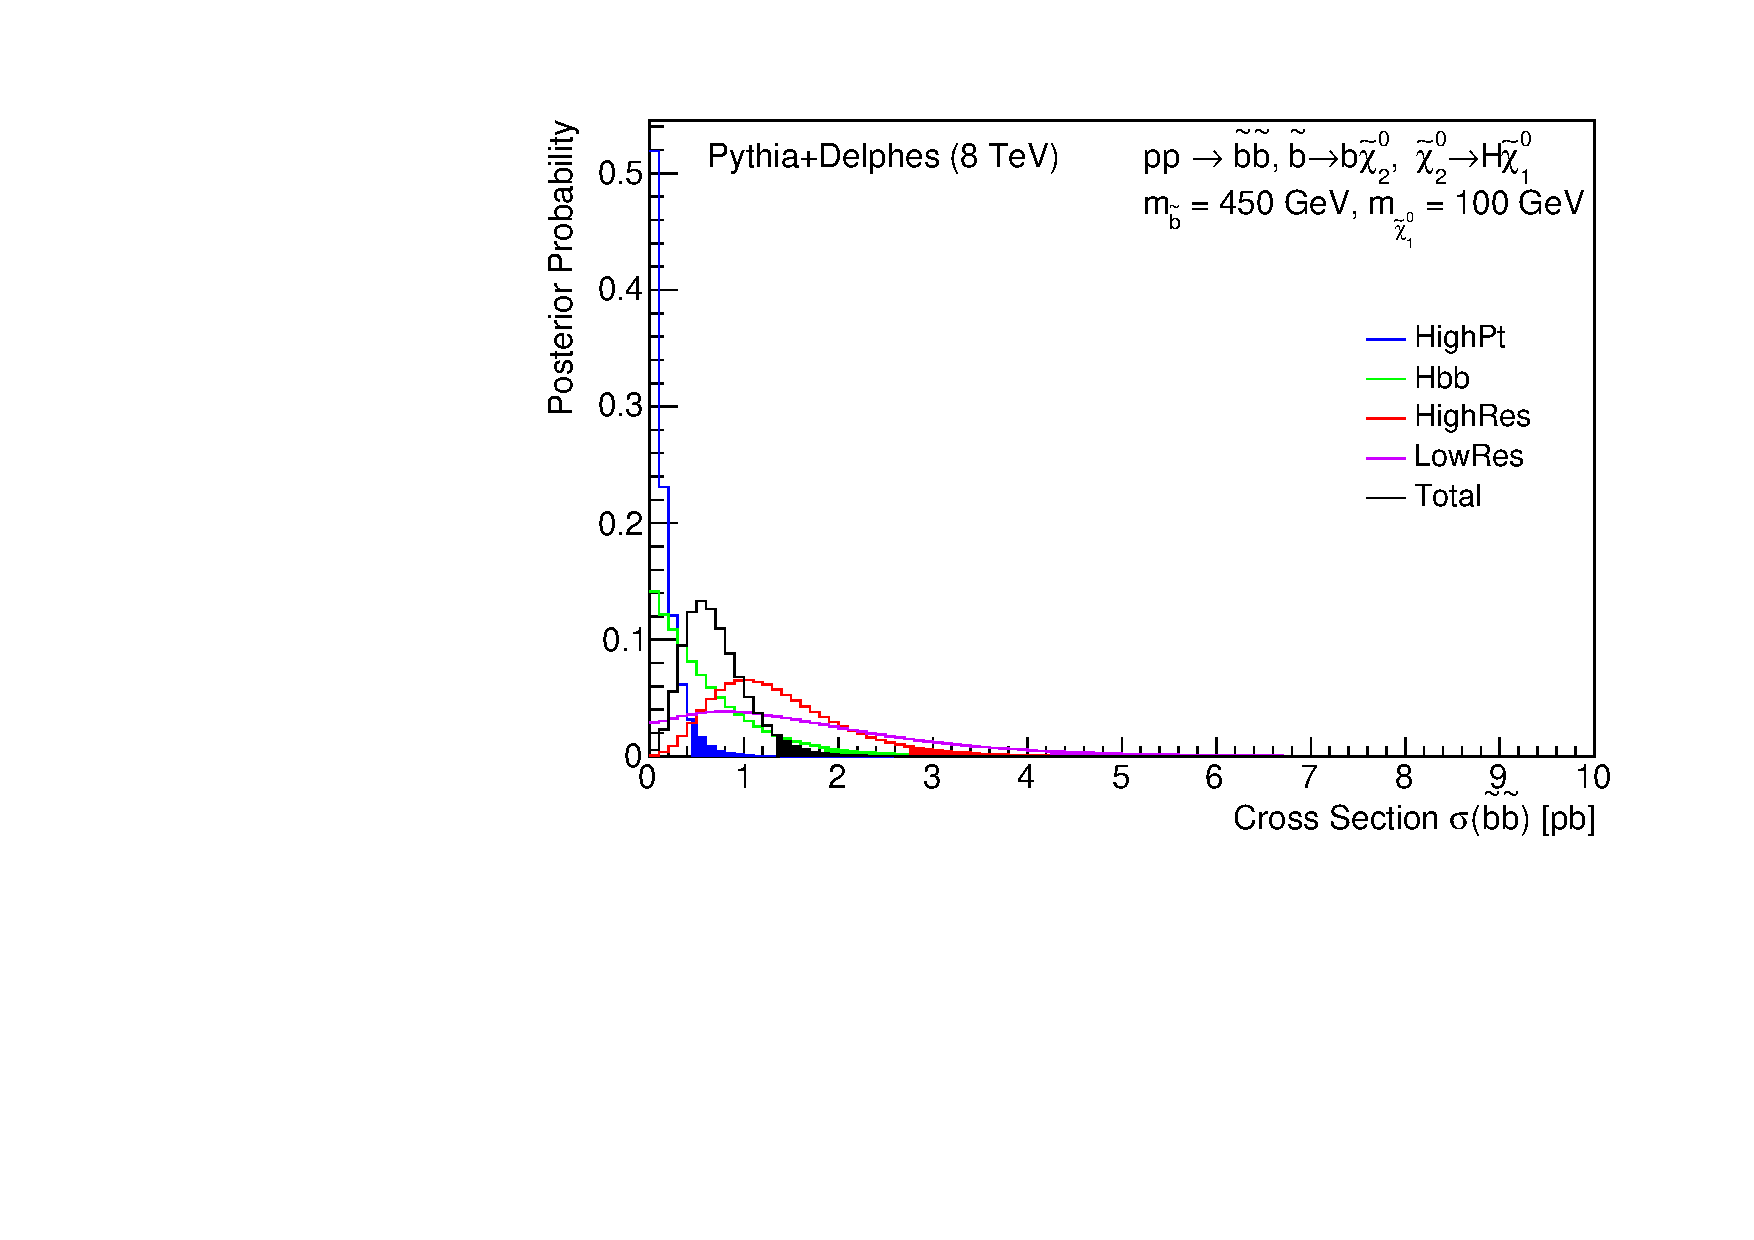
\includegraphics[width=0.45\textwidth]{figs/pheno/posterior_T2bH_450_100.pdf}
%\caption{\label{fig:T2bHPosterior450} Posterior probability
% density functions for the $\sbottom_1\sbottom_1$ production cross
%  section in model B for the \texttt{HighPt} box (blue),
%  \texttt{HighRes} box (red), \texttt{Hbb} box (green), and the combination (black). The solid colored region
%  under each curve illustrates the 5\% tail probability. Note, the chosen masses are $m_{\tilde\chi_1^0}=100$~GeV and
%  $m_{\tilde{\chi}_2^0}=230$~GeV.}
%\end{figure}

\begin{figure}[htb]
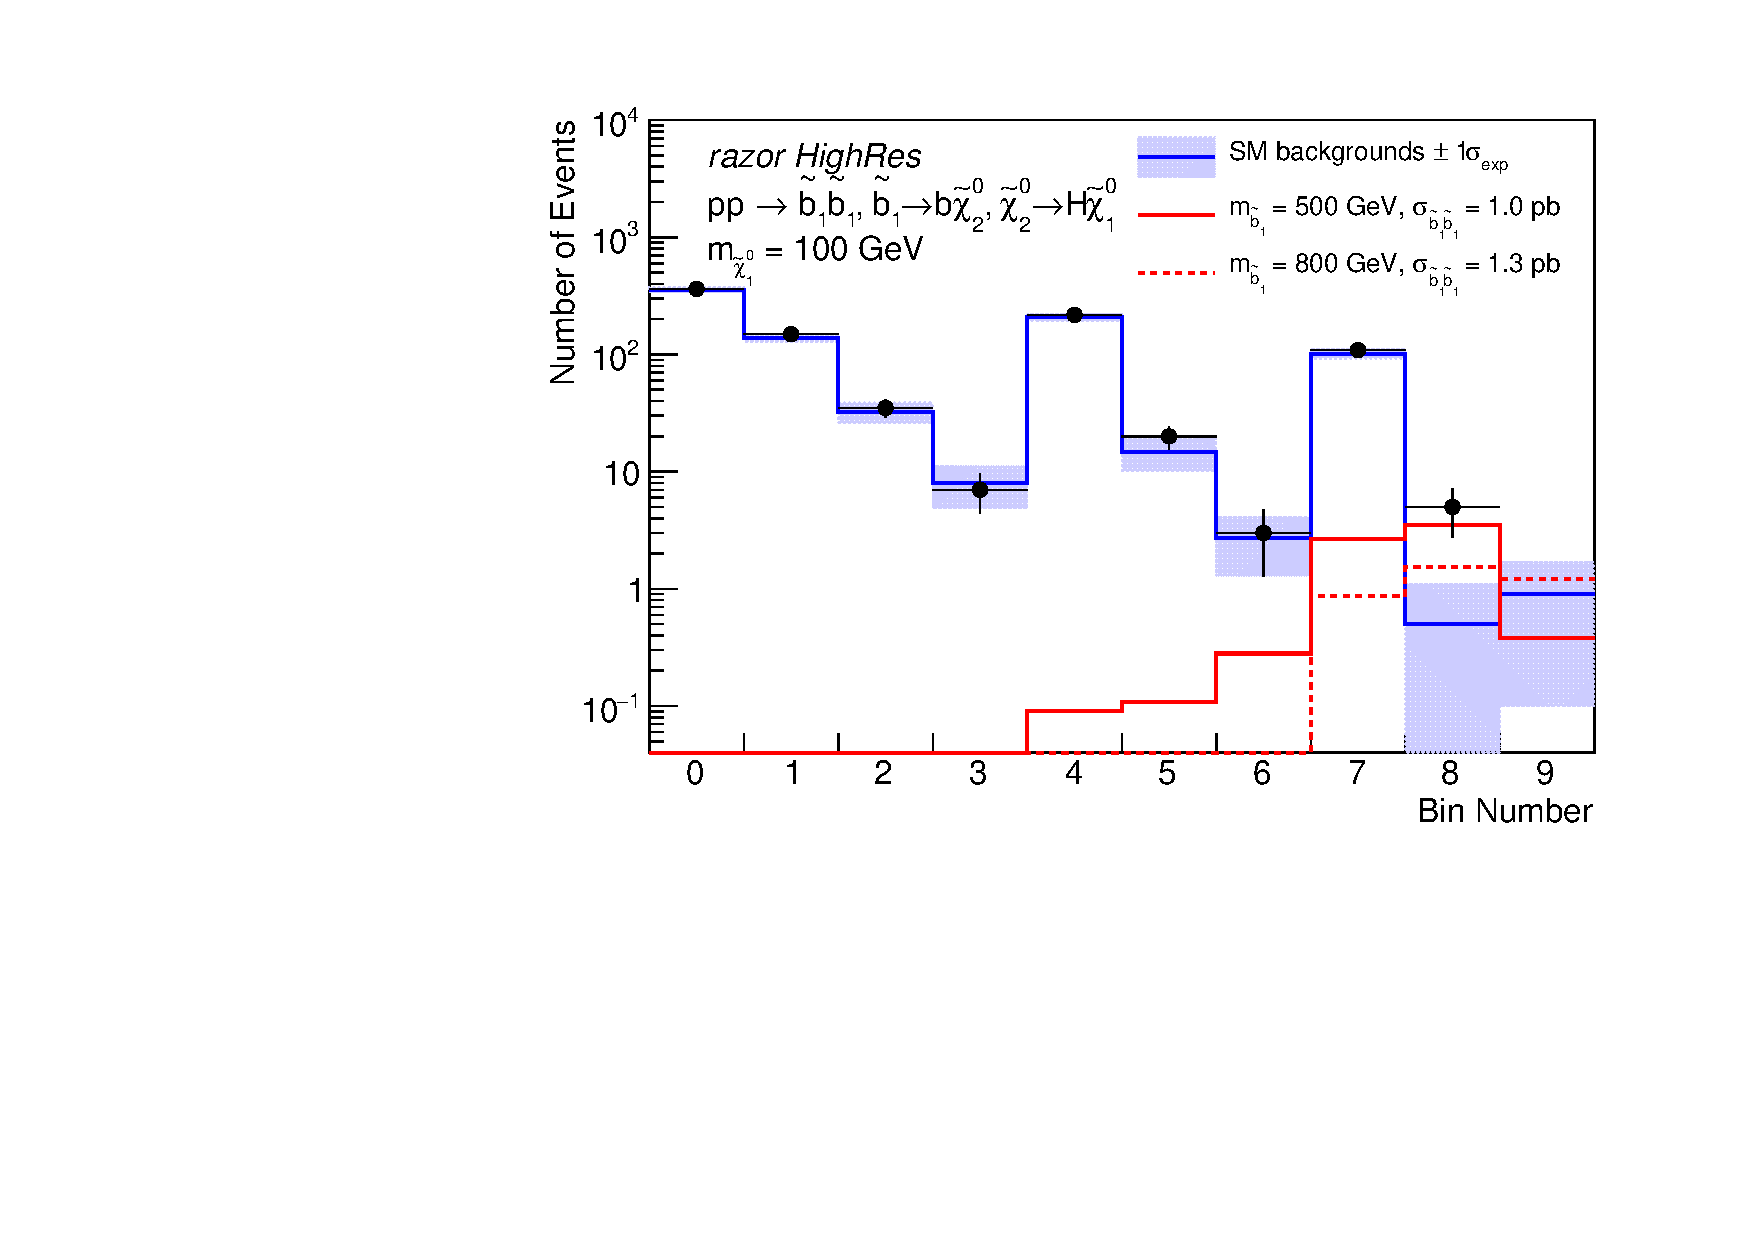
\includegraphics[width=0.45\textwidth]{figs/pheno/obsexp_T2bH_HighRes.pdf}
\caption{\label{fig:T2bHExpObs500800} The expected background and
  uncertainty compared to the ``best-fit'' signal distribution in the \texttt{HighRes} box for two particular
  mass points, $m_{\sbottom_1}=500$~GeV and $m_{\sbottom_1}=800$~GeV, in model B.}
\end{figure}

\begin{figure}[htb]
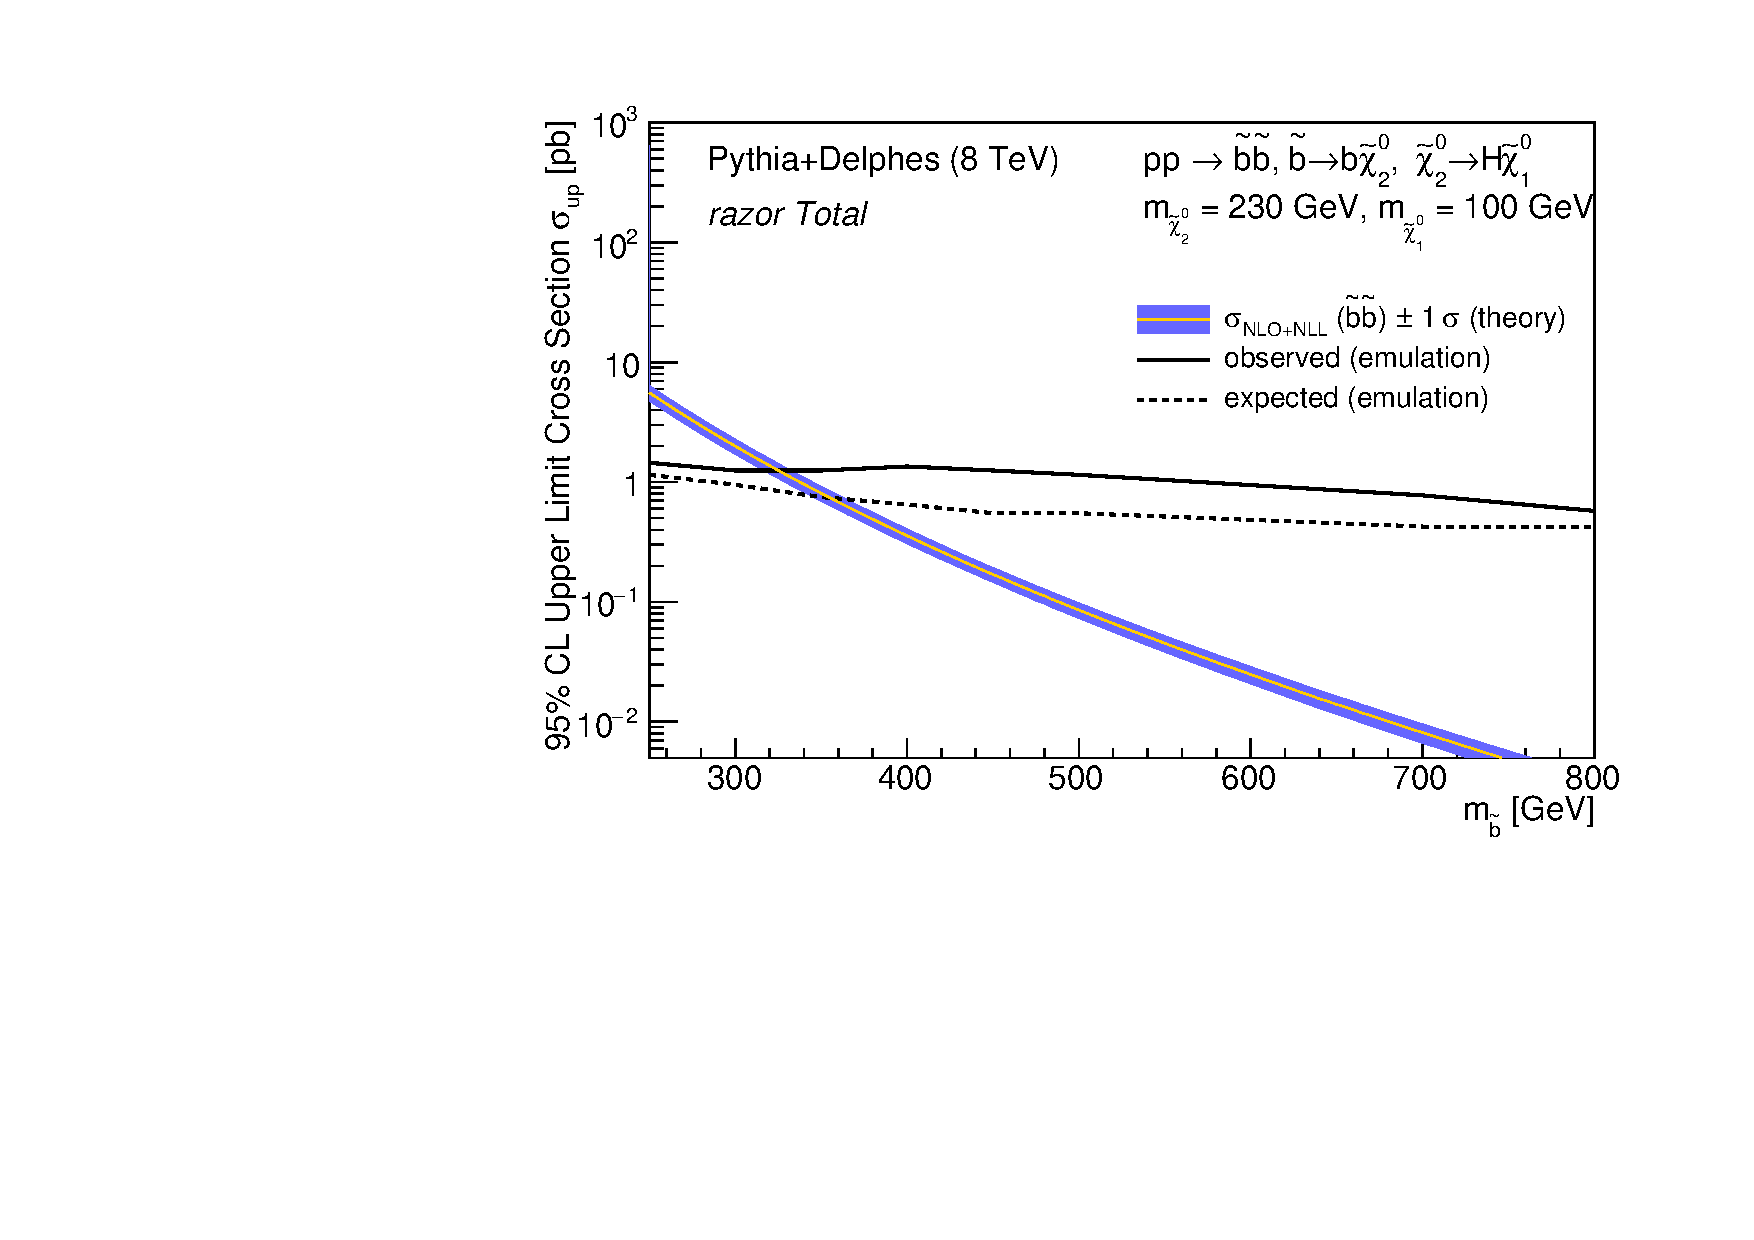
\includegraphics[width=0.45\textwidth]{figs/pheno/xsecUL_T2bH_100_Total.pdf}
\caption{\label{fig:T2bH1dLimit} The 95\% CL upper limit on the
  cross section on $\sbottom_1\sbottom_1$ production in model B as a function of $m_{\sbottom_1}$ (black) compared
  to the NLO+NLL predicted cross section (yellow). Note, this scan assumes
  $m_{\tilde\chi_1^0}=100$~GeV and $m_{\tilde{\chi}_2^0}=230$~GeV.}
\end{figure}

\begin{figure}[htb]
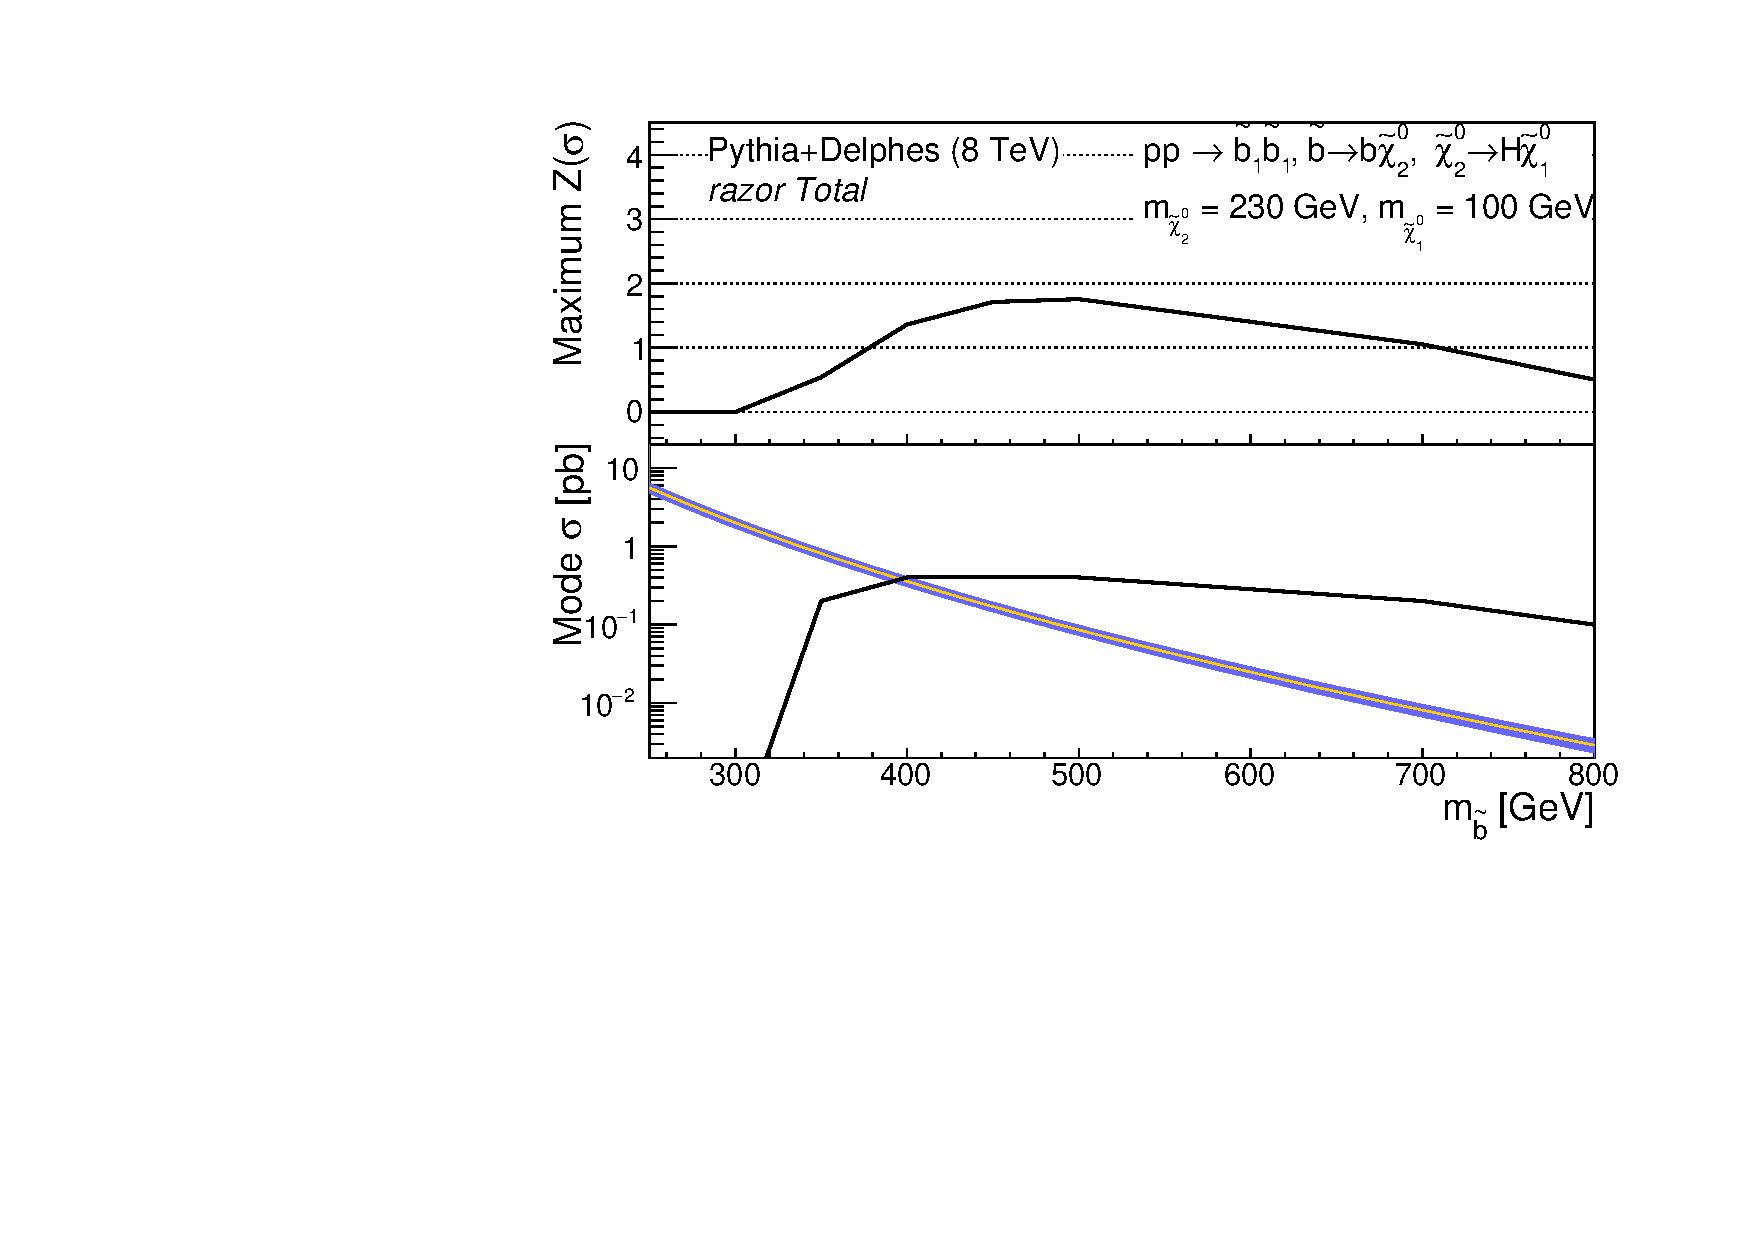
\includegraphics[width=0.45\textwidth]{figs/pheno/signif_T2bH_100_Total.pdf}
\caption{\label{fig:T2bH1dSignif} The maximum significance $Z$ for a
  given $m_{\sbottom_1}$ (top) and the ``best fit'' signal cross
  section (bottom) compared to the NLO+NLL predicted cross section (yellow). Note, this scan assumes
  $m_{\tilde\chi_1^0}=100$~GeV and $m_{\tilde{\chi}_2^0}=230$~GeV.}
\end{figure}


\section{Conclusions}
\label{sec:conclusions}